\section{Dataset Characterization}
\label{sec:char}

In this section we carry out our analysis of the Docker Hub dataset by characterizing
layers (\S~\ref{sec:layers}) and images (\S~\ref{sec:images}) based on
the above presented metrics. While overall we are interested in its general structure,
we also analyze specific properties that allow us to draw conclusions regarding the
caching, compression, and provisioning.

As shown in Figure~\ref{fig_image_growth}, the number of repositories increased
linearly during our observation period from May 30th to September 20th
2017. Note that the graph shows a gap of \gap days due to Docker Hub changing the way it
indexes repositories. The total number of repositories
grew from 633,915 to 687,292, resulting in an average creation rate of 1,241
repositories per day. This rapid growth shows that storage optimizations will
be crucial for the registry in the future.

%
%\paragraph{Docker Hub growth}
%%
%Figure~\ref{fig_image_growth} shows the linear
%growth in the number of repositories in Docker Hub from May 30 to September 20,
%2017.
%%
%%As discussed in~\cite{XXX}, Crawler searched for `/' by using Docker hub
%%search engine, crawled the web page, and obtained the total number of
%%non-official public repositories in Docker hub each day. By summing both
%%official repository count and non-official repository count, we got the total
%%number of repositories in Docker hub each day.
%%
%During this 110-day period the total number of repositories increased by 53,337
%from 633,915 to 687,292, resulting to the average creation rate of 1,241
%repositories daily.
%%
%The graph is missing the points between July 11 and July 26 because Docker Hub
%stopped indexing ``/'' symbol in the repository names (which we originally used
%to search for all repositories).
%%
%We noticed this issues on July 26 and started to use ``*'' symbol instead.


\begin{figure}
  \centering
  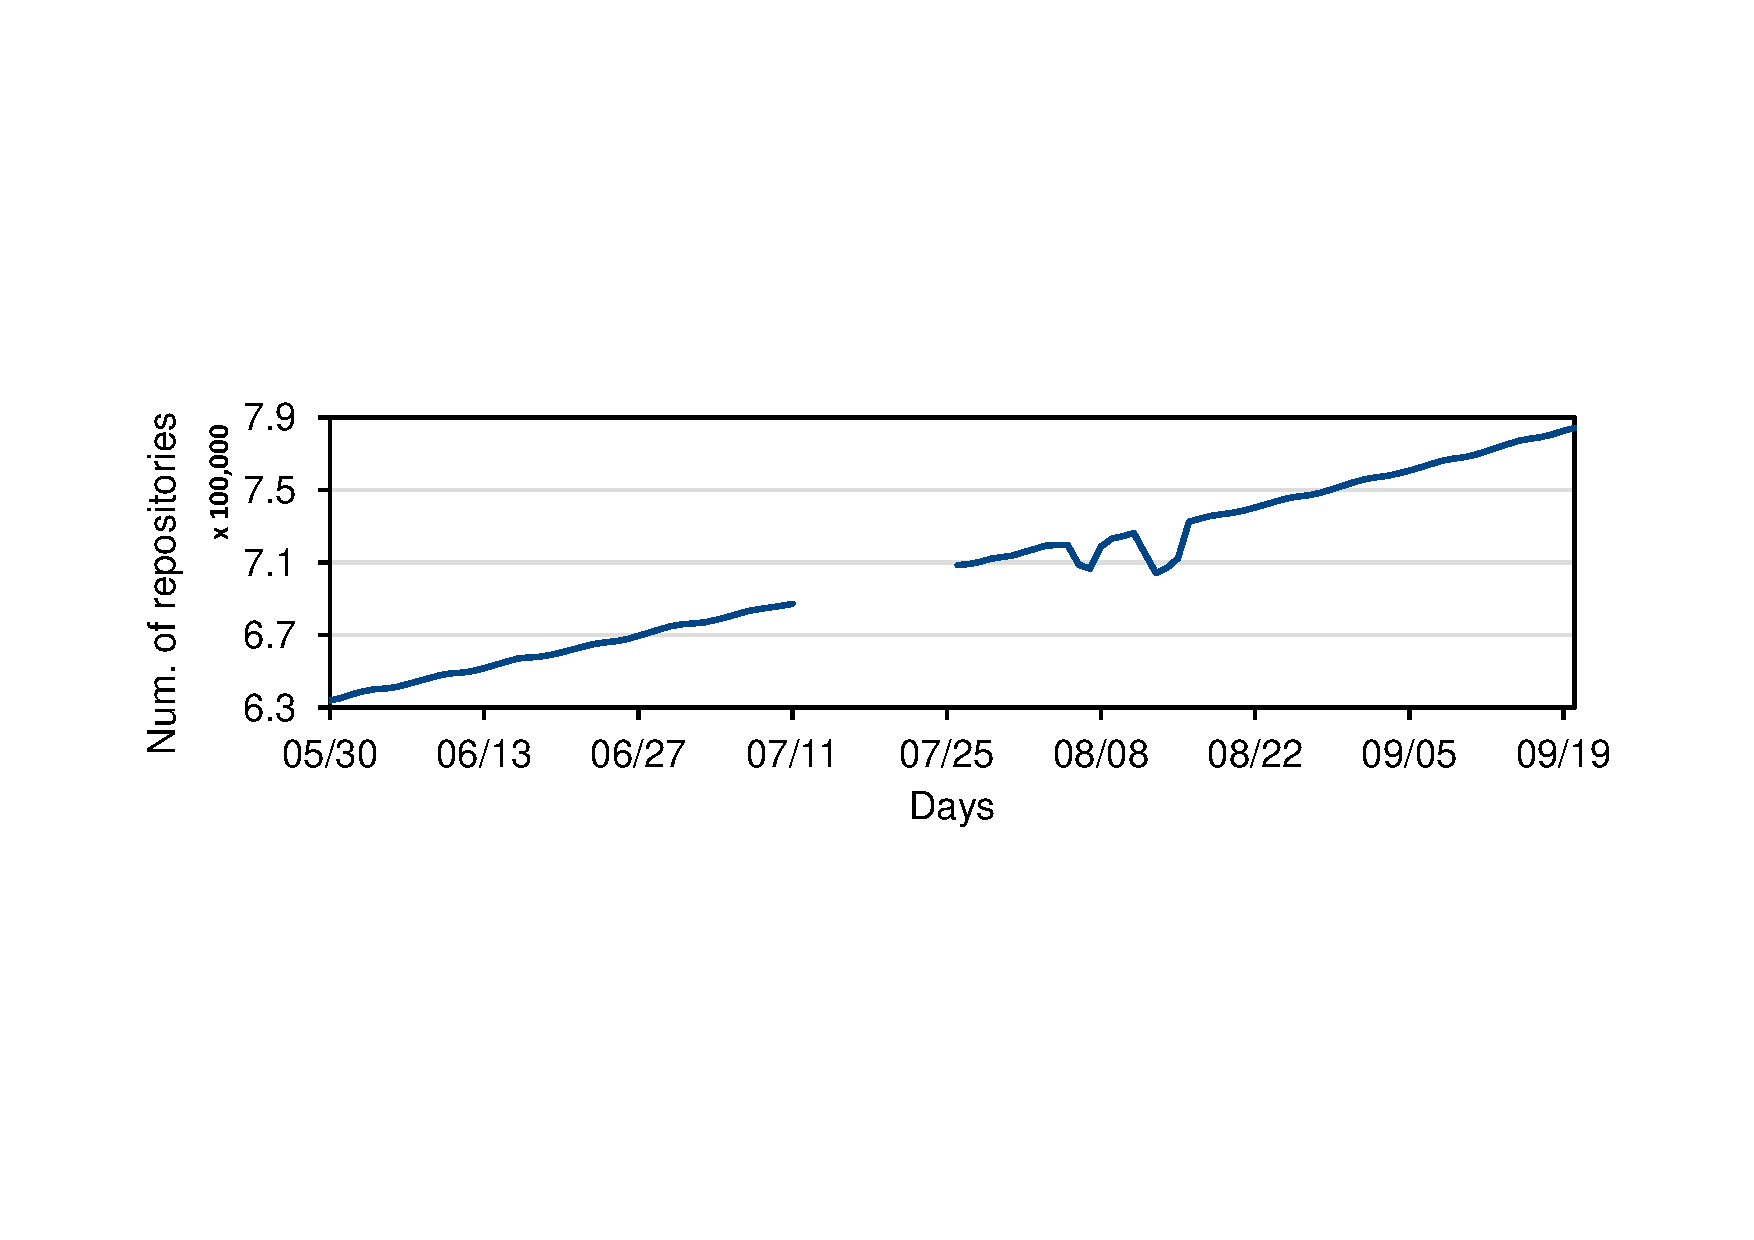
\includegraphics[width=0.5\textwidth]{graphs/image_growth.pdf}
  \caption{Total number of public repositories in Docker Hub
	   from May 30 to September 20, 2017. Y axis starts
	   at 630,000 repositories.
	   \vcomment{X axis label should be ``Date''.\nancomment{addressed all}}
	   \vcomment{Y axis label x100,000 ``is badly aligned''.}
	   \vcomment{Y axis label x100,000 ``is badly aligned''.}
	  }
  \label{fig_image_growth}
\end{figure}

\subsection{Layers}
\label{sec:layers}

%\nancomment{could remove archival size from all sections}
We start by analyzing layers in terms of size and compressibility, and file and directory
counts and directory depths.

%%%%%%%%%%%%%%%%%%%%%%%%%%%%%%%%%%%%%%%%%%%%%%%%%%%%%%%%%%%%%%%%%%%%%

\begin{figure}[!t]
	\centering
	\subfigure[CDF of layer sizes]{\label{fig_layer_size_cdf}
		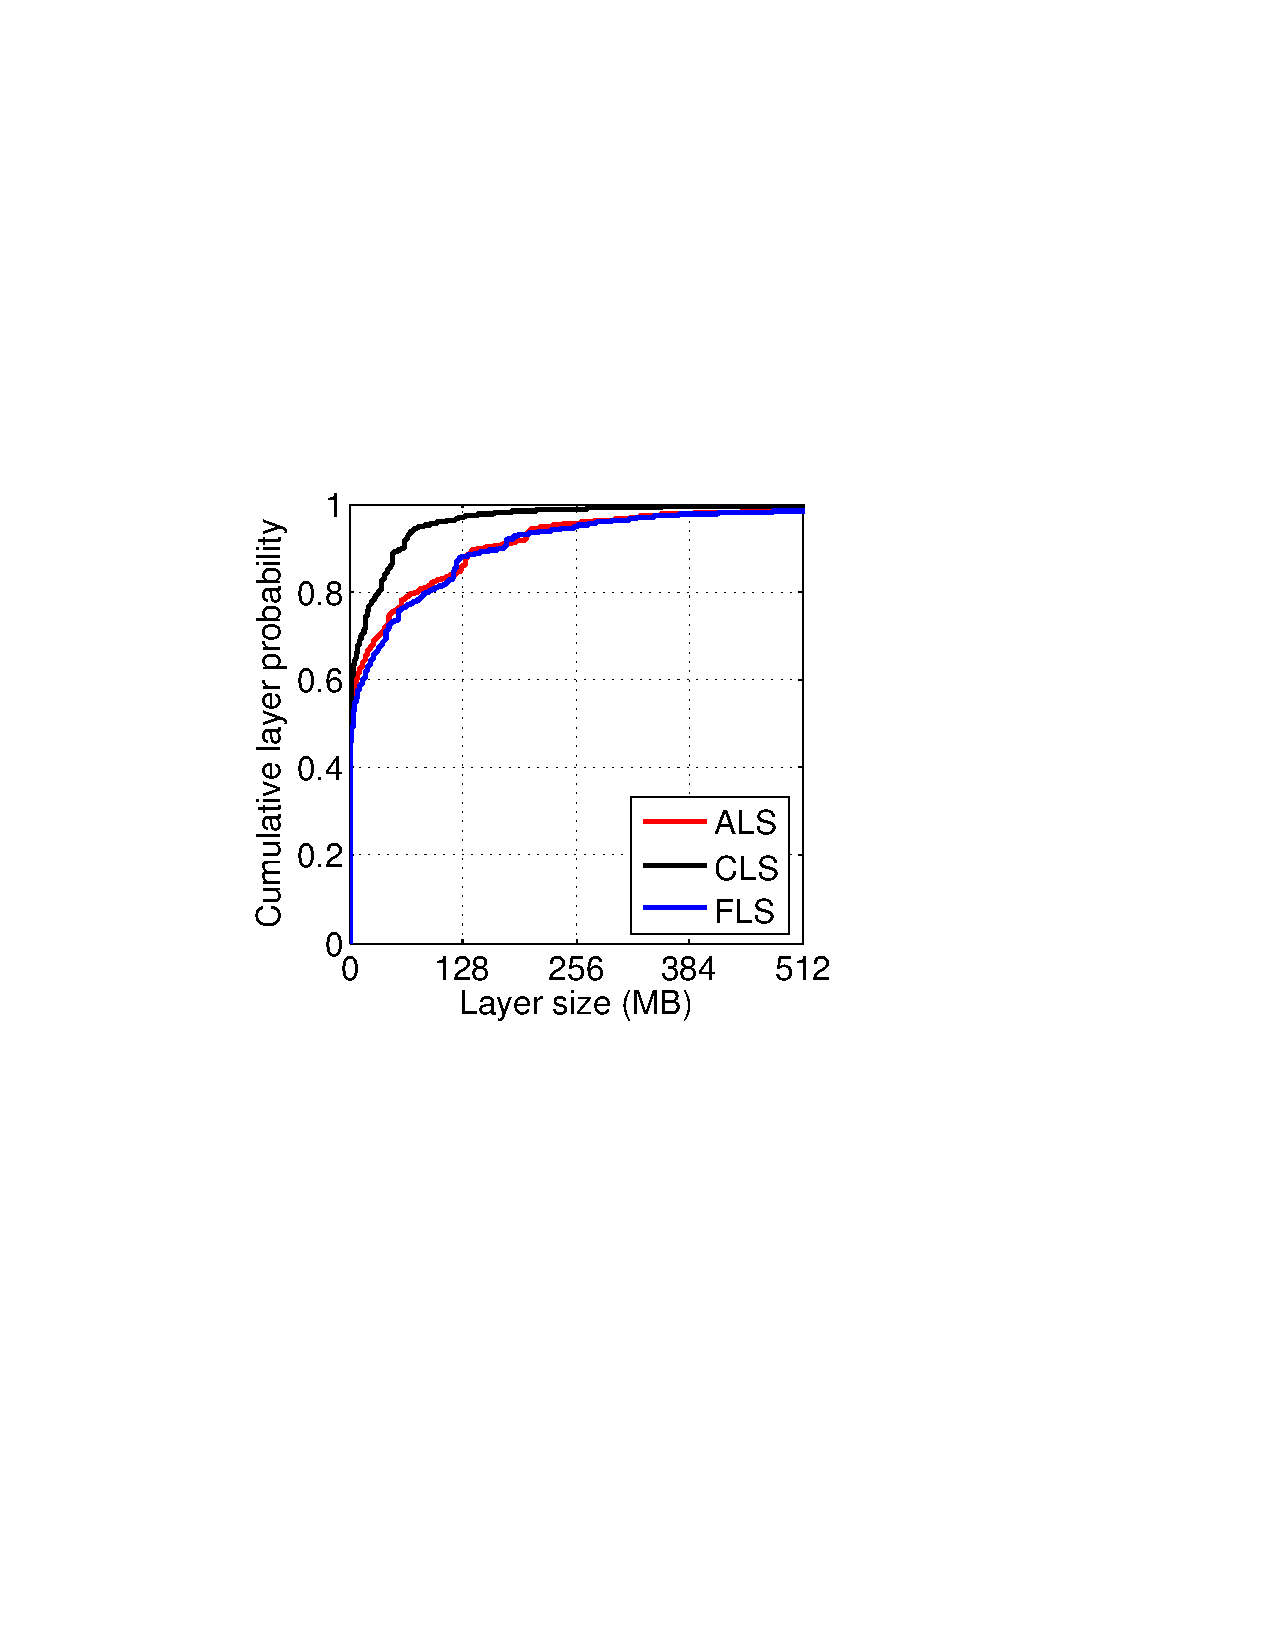
\includegraphics[width=0.234\textwidth]{graphs/layer_size_mb.pdf}
	}
	\subfigure[Histogram of layer sizes]{\label{fig_hist_layer_size}
		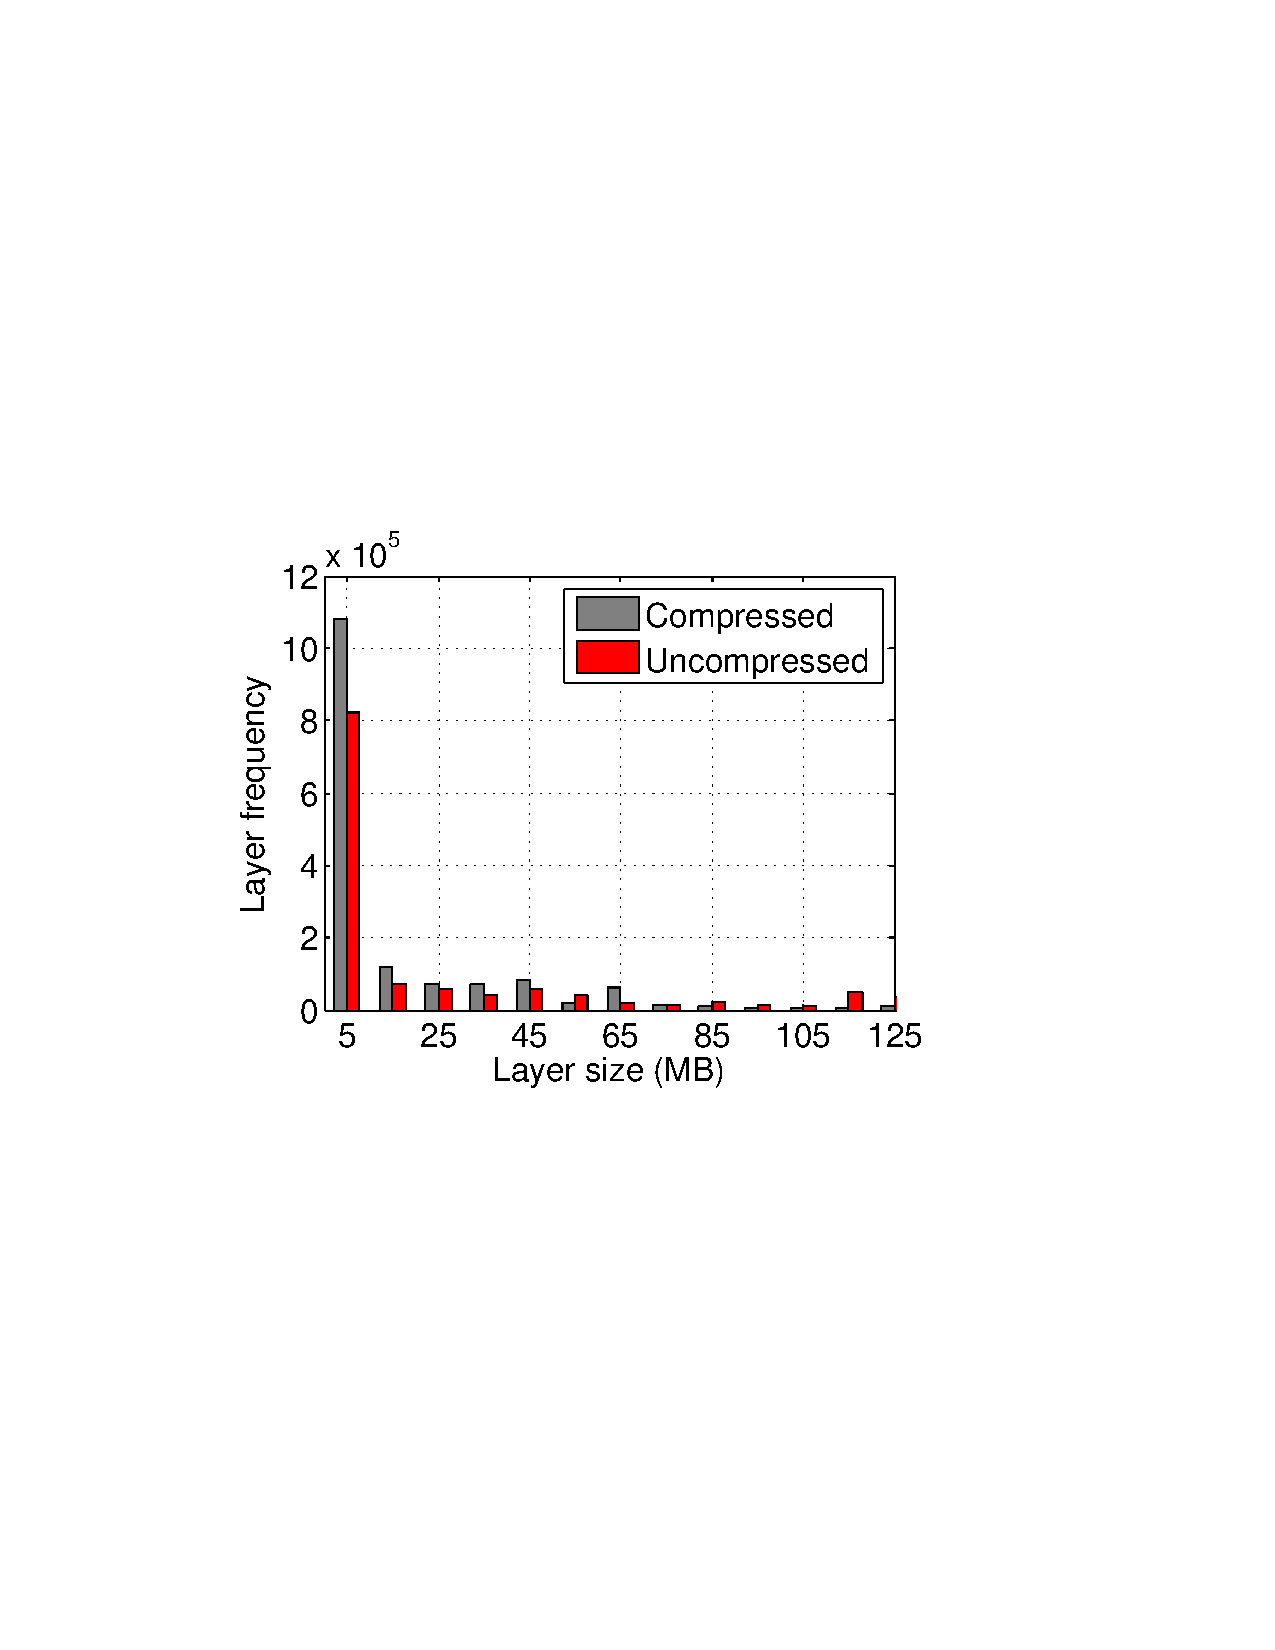
\includegraphics[width=0.213\textwidth]{graphs/hist_layer_size.pdf}
	}
	\caption{Layer size distribution
	\vcomment{Let's use CLS, ALS, and FLS abreviations\nancomment{addressed}}.
	\vcomment{CLS size should go first}.
	\vcomment{We need to use different types of lines (solid, dotted, etc.)
		or markers (round, triangular)}.
	\vcomment{In figure B it is not clear to which bar group corresponds
		  to which layer size. I suggest to try to rotate the graph
		  by 90 grads to fit all layer size labels.\nancomment{aligned label with bar}}
	}
	\label{fig-layer-size}
\end{figure}


\paragraph{Layer sizes}
%
We characterize layer sizes using two different different metrics:
%
1)~Compressed Layer Size (CLS)---the format a layer is stored in the registry or
transferred to a client;
%
%2)~Archived Layer Size (ALS)---layer in decompressed but archived format;
%
and 2)~Files in Layer Size (FLS)---the sum of the size of the uncompressed files contained
in the layer.
%
Figure~\ref{fig_layer_size_cdf} shows the CDF of the two metrics.


%The ALS and FLS curves are, expectedly, close to each other (within 5\% for
%any given layer size) while compressed layers are typically smaller.
%j
We see that 90\% of the layers are smaller than 177~MB in uncompressed 
format and smaller than 63~MB in compressed format.
%
Interestingly, about half of the layers are smaller than 4~MB, independent
of the format. That means that the registry stores a large number of
small layers which cannot benefit from compression.
%
\nancomment{I removed the following lines because we analyzed all layers.}
%As we described earlier in \S~\ref{sec:methodology}, we only
%analyzed layers smaller than 2~GB in compressed format. This
%resulted in the largest analyzed uncompressed layer being
%of \gap~GB large.
%
%\vcomment{need to adjust Methodology to reflect this.}

To analyze the actual numbers, we zoom into the 0--128~MB range
(see Figure~\ref{fig_hist_layer_size}).
%
More than 1 million and 800,000 layers are smaller than 5~MB
in compressed and uncompressed format, respectively. After that,
the frequency drops rapidly and we only see around 100,000 layers
between 5~MB and 15~MB.

\begin{figure}[!t]
	\centering
	\subfigure[CDF of compression ratio]{\label{fig_cdf_compression_ratio}
		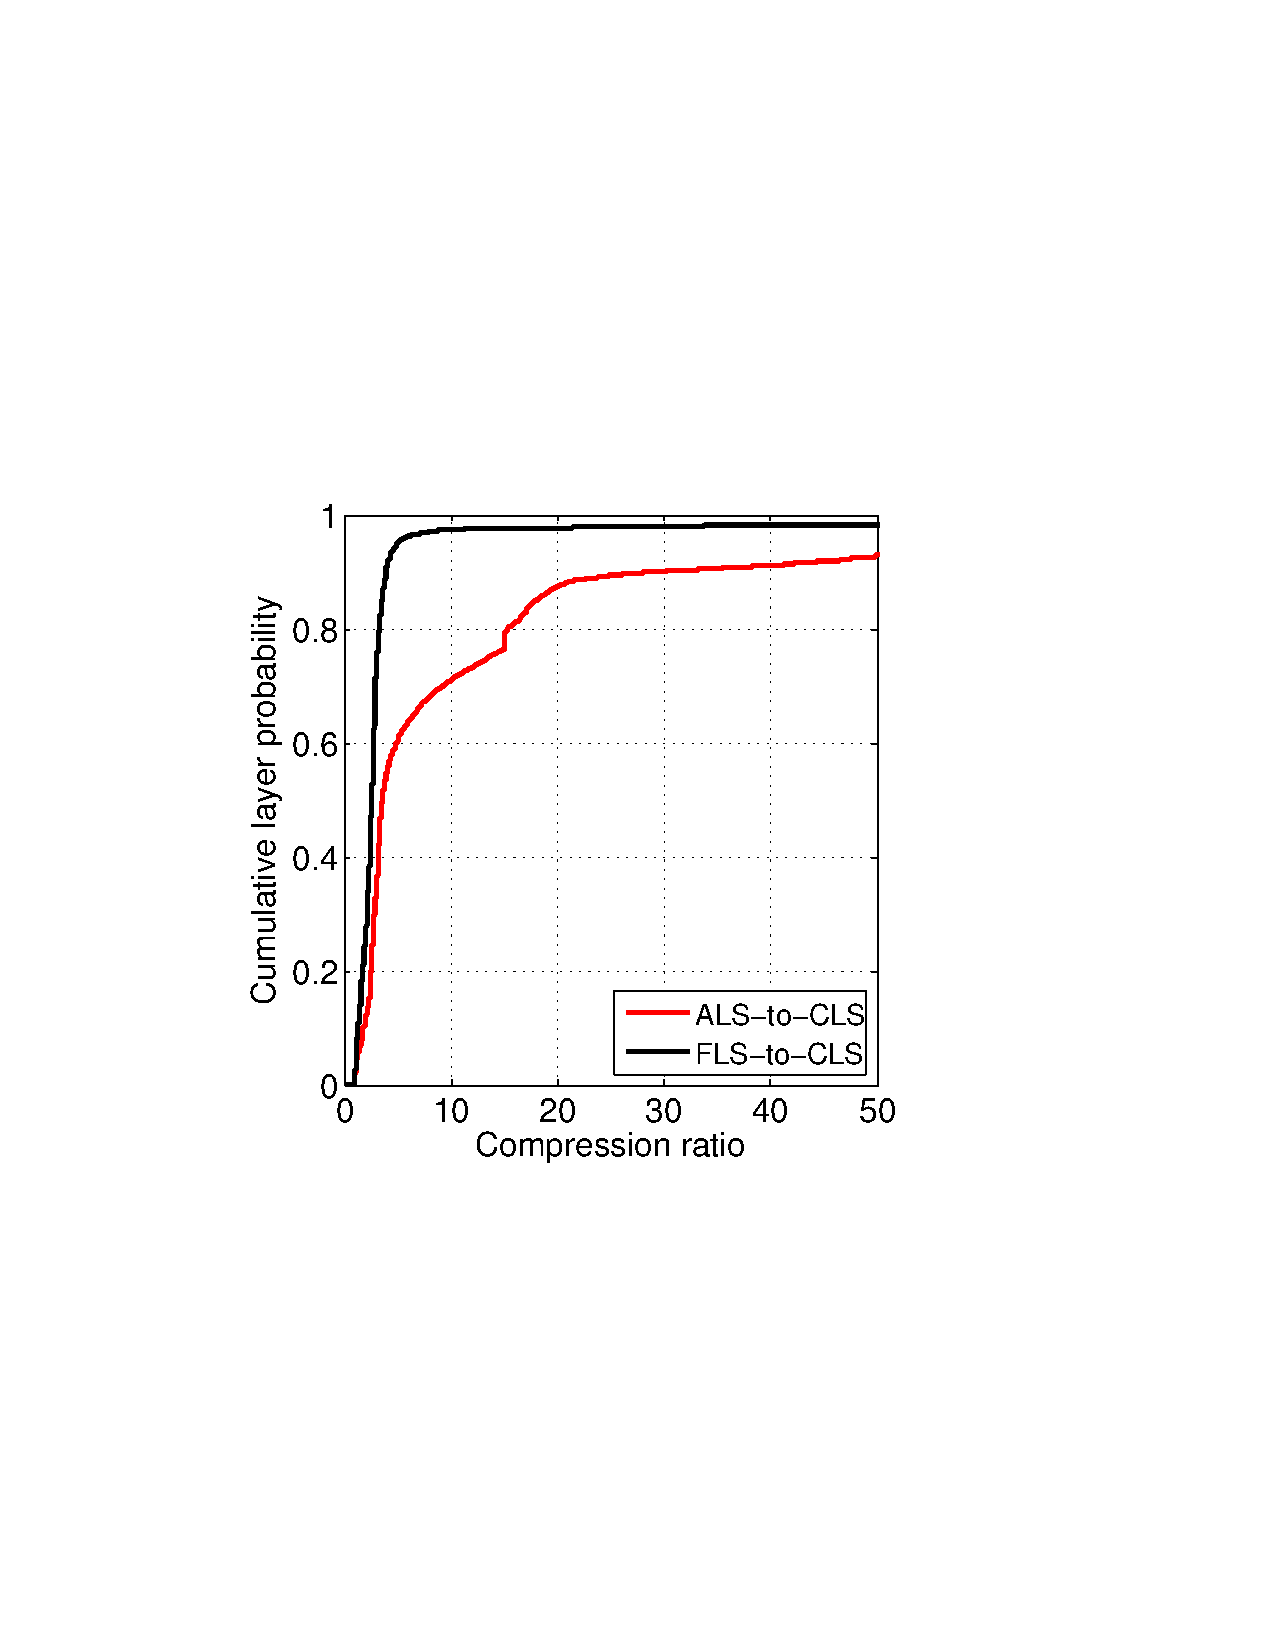
\includegraphics[width=0.23\textwidth]{graphs/cdf_compression_ratio.pdf}
	}
	\subfigure[Histogram of comp. ratios]{\label{fig_his_compression_ratio}
		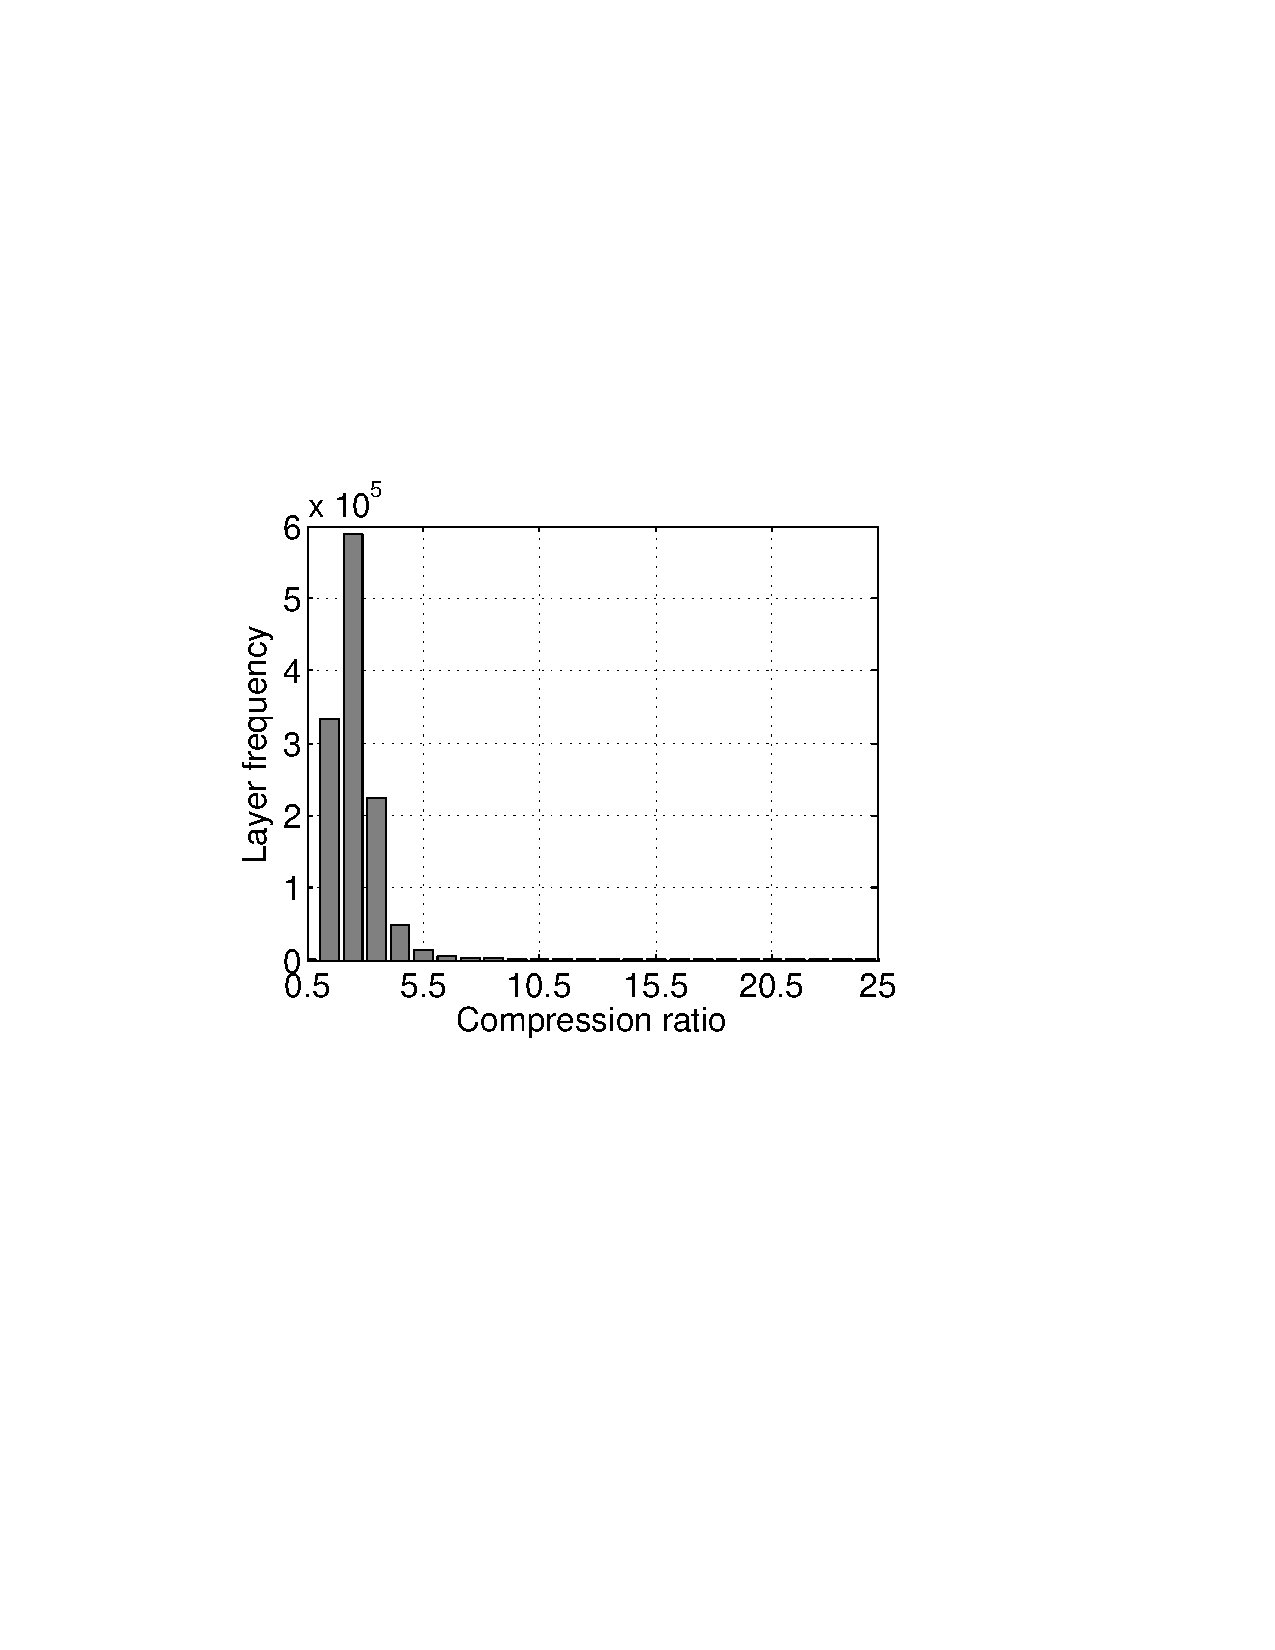
\includegraphics[width=0.223\textwidth]{graphs/his_compression_ratio.pdf}
	}
	\caption{Layer compression ratio distribution
	%\vcomment{Different colors are used in figure (a) and (b) FLS/CLS\nancomment{will address later}}
	}
	\label{fig-compression-ratio}
\end{figure}


%\paragraph{Layer compression ratios}

To further study the sizes and the impact of compression, we calculate
the FLS-to-CLS compression ratios (see Figure~\ref{fig_cdf_compression_ratio}).
%
%The ALS-to-CLS ratio is generally greater than the FLS-to-CLS ratio
%because small files in layers get larger when combined in a tar archive.
%
90\% of layers have a  CLS-to-FLS ratio less than 4 and the median
compression ratio is 2.6. The largest compression ratio is 1026.
%
%Half of the layers have a compression ratio (both ALS-to-CLS and
%FLS-to-CLS) around 3.
%
%
%The maximum FLS-to-CLS is 512,930 and maximum ALS-to-CLS is 1026.
%
Looking at the histogram (see Figure~\ref{fig_his_compression_ratio}), we see
that around 600,000 layers have a compression ratio of between 1.5 and 2.5\nancomment{it is between 2 and 3} while more than
300,000 between 0.5 and 1.5\nancomment{it is between 1 and 2}.
%
%Two peaks in the graph correspond to 587,000 layers that have the FLS-to-CLS ratio of 3
%and 331,000 layers that have the ALS-to-CLS ratio of 3.

Our size analysis reveals an interesting trade-off. Compression is computationally
expensive and is one of the major sources of latency when pulling an image from Docker Hub.
As the majority of layers is small and has low compression ratios, it can
be beneficial to store small layers uncompressed in the registry to reduce pull latencies.

%%%%%%%%%%%%%%%%%%%%%%%%%%%%%%%%%%%%%%%%%%%%%%%%%%%%%%%%%%%%%%%%%%%%%

\begin{figure}
	\centering
	\begin{minipage}{0.23\textwidth}
		\centering
		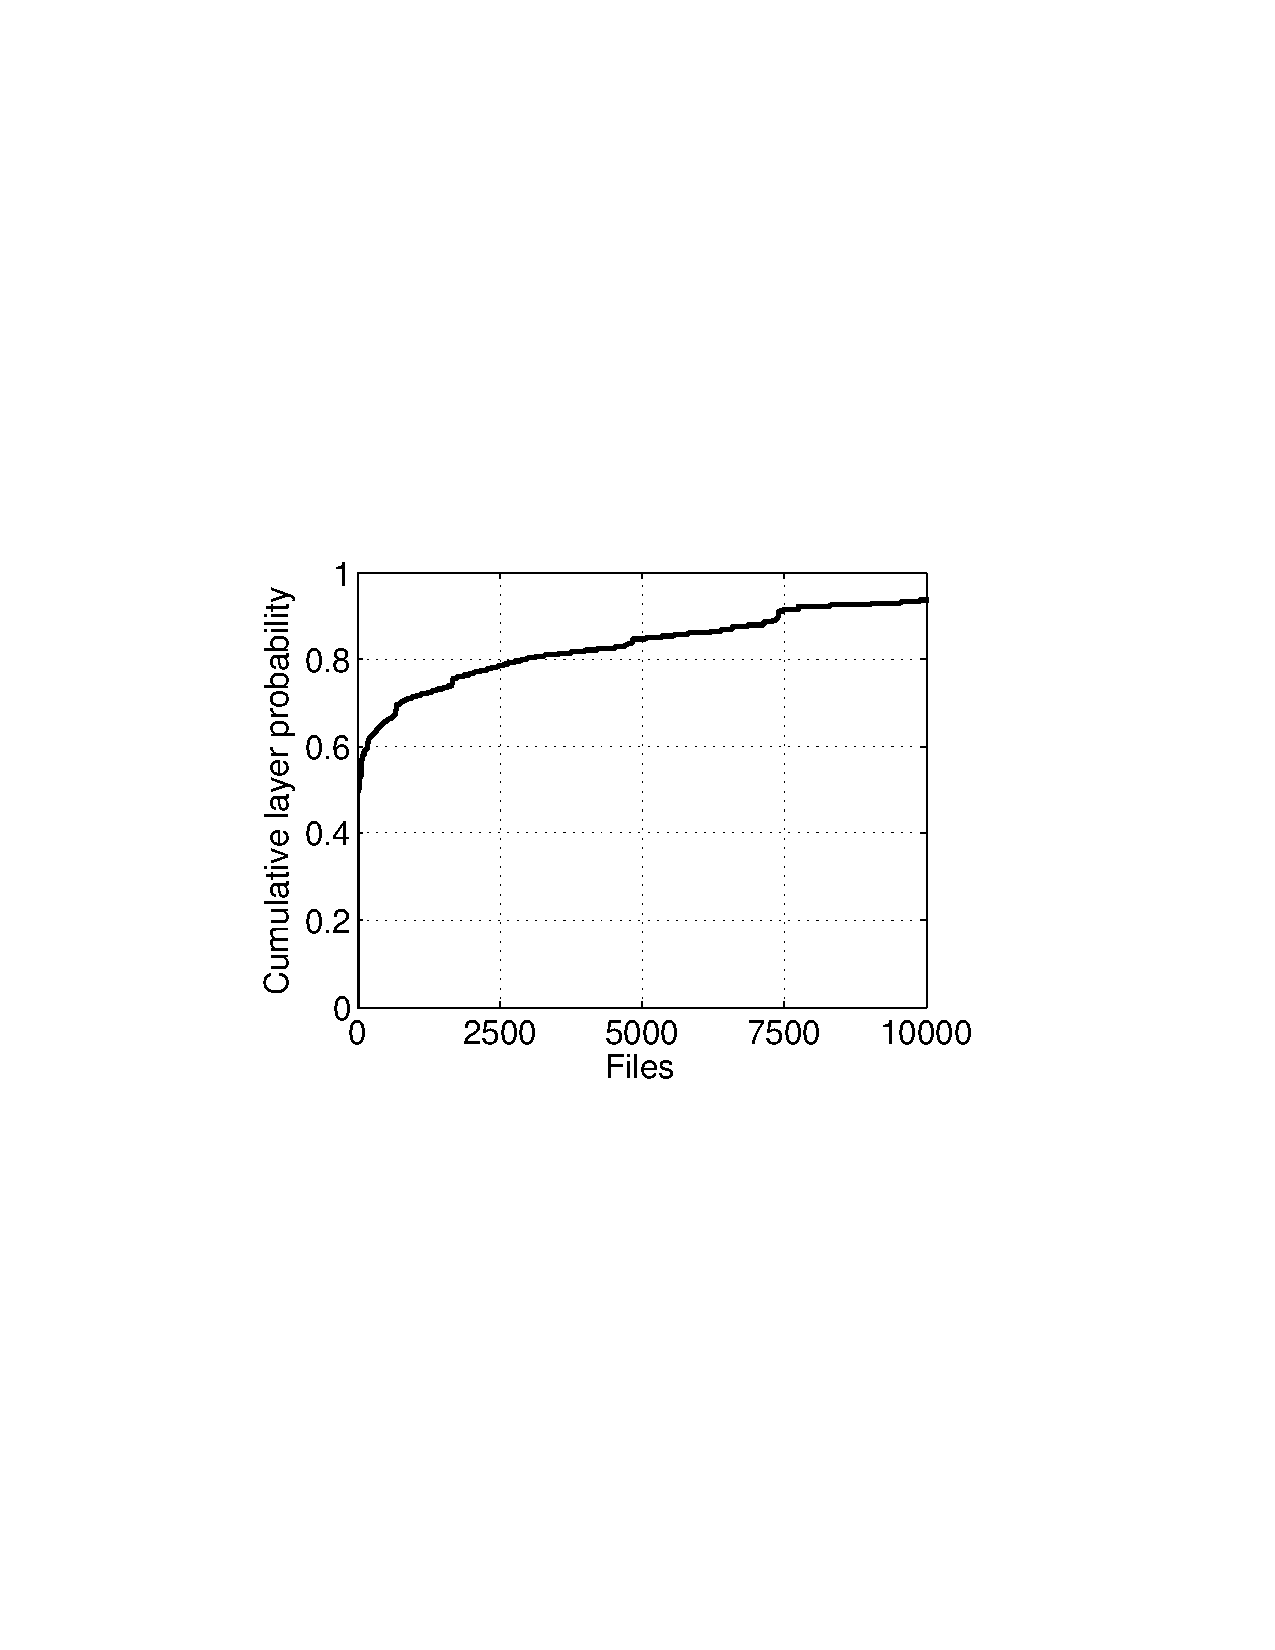
\includegraphics[width=1\textwidth]{graphs/file_cnt.pdf}
		\caption{File count distr.}
		\label{fig_file_cnt}
	\end{minipage}
	\begin{minipage}{0.23\textwidth}
		\centering
		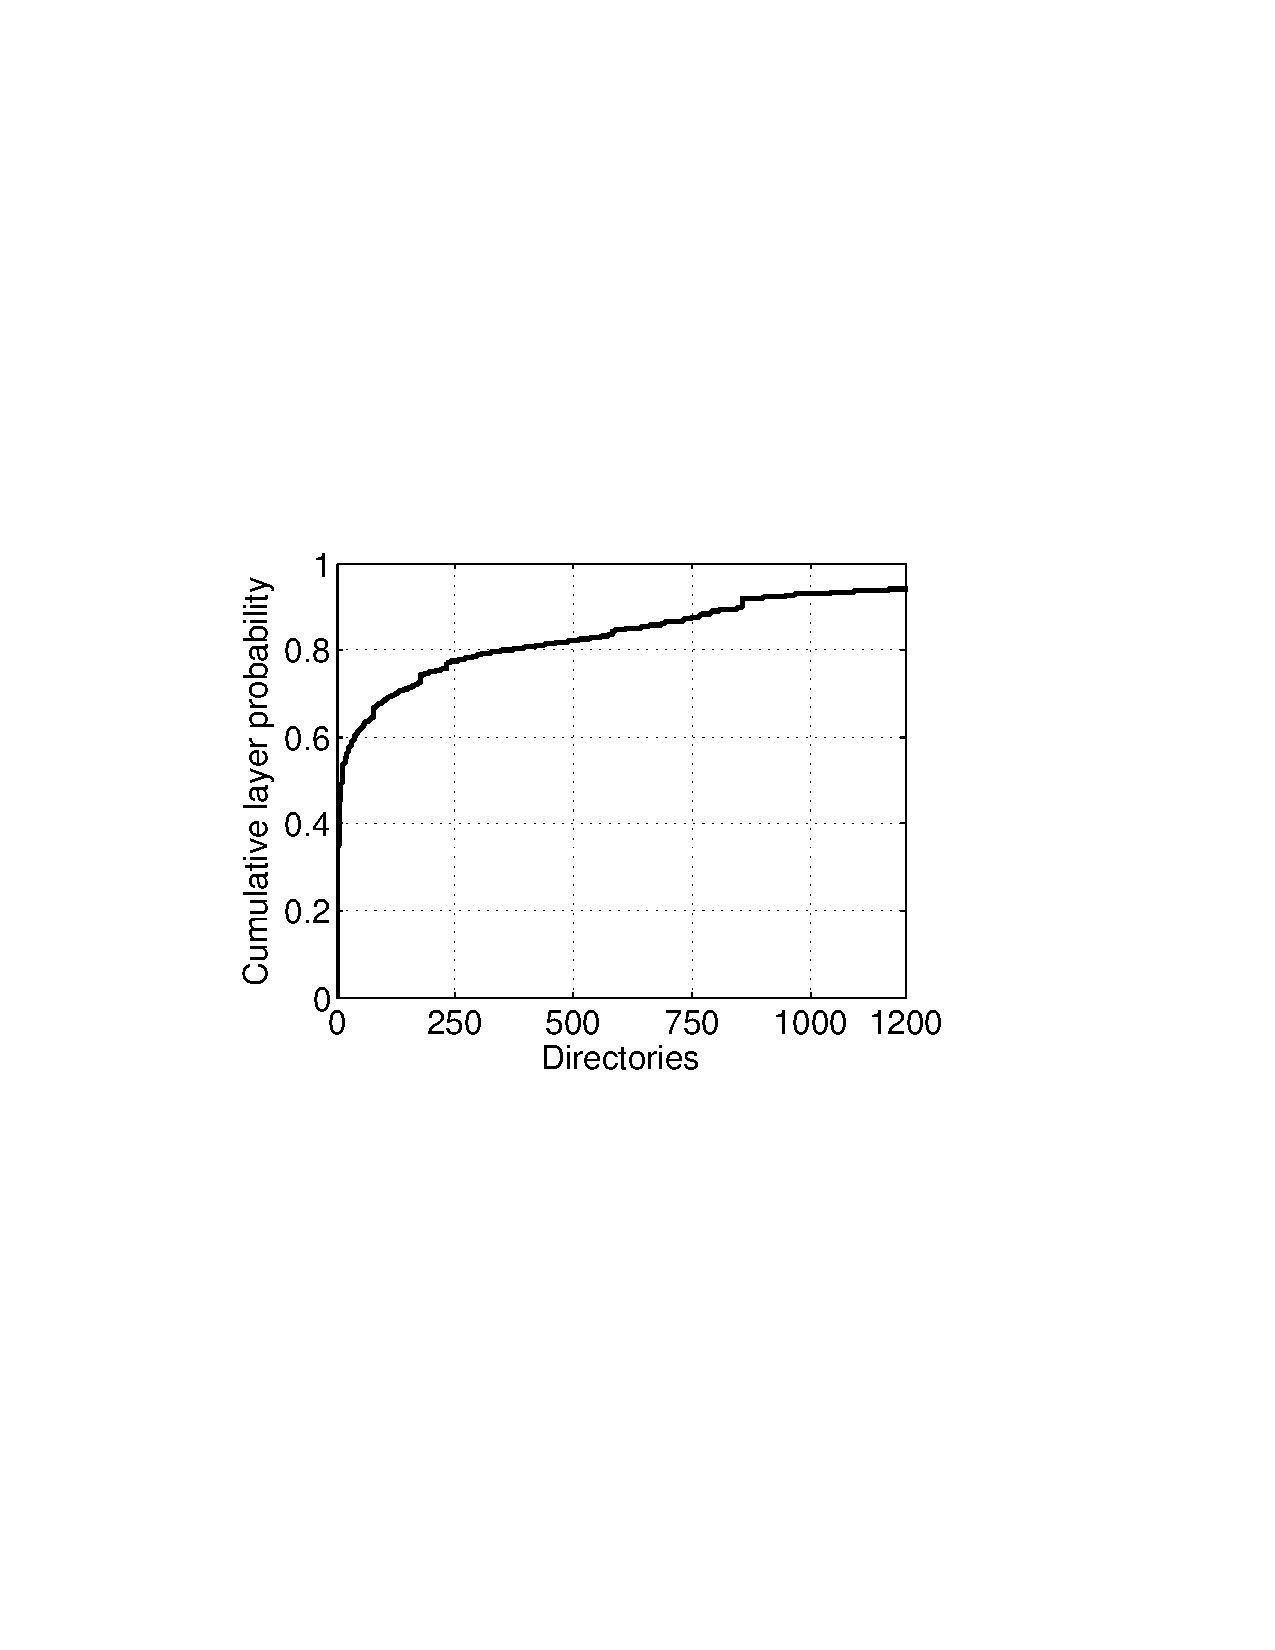
\includegraphics[width=1\textwidth]{graphs/dir_cnt.pdf}
		\caption{Dir. count distr.
		%\vcomment{Let's make thise figure subfigures.}
		}
		\label{fig_dir_cnt}
	\end{minipage}%
\end{figure}
%

\paragraph{File and directory counts}

Next, we look at file and directory metrics in layers.
Figure~\ref{fig_file_cnt} and~\ref{fig_dir_cnt} show the CDFs of file
and directory counts in all layers, respectively.
%
The results show that 90\% of layers contain less than 7,410 files while half
of the layers have less than 30 files.
%
We also found that 27\% of the layers only have a single file while 7\% even showed
no files at all. We currently do not know the exact reason for the empty layers but
plan to investigate their corresponding images in the future\nancomment{The layers are not empty since it could have directories}. On the other hand,
the largest layer contains 826,196 files which was part of a Debian image.
%
%The average is 2,200.
%
For directories, 90\% of the layers have less than 826 directories and half of the layers consist
of less than 11 directories. We again observe a wide range with a minimum of a single directory
and a maximum of 111,940. The layer with the most directories was part of
the \textit{conjurinc/developer-quiz} image.

%\paragraph{Directory depths}

%After extracting and unpacking gzip compressed layer archival files,
Besides the count, we also calculate the maximum directory depth for every layer
(see Figure~\ref{fig_layer_depth}).
%
Around 90\% of all layers have a directory depth less than 10
while for 50\%  of the layers, the directory depth is less than 4. 
%
The most frequent directory depth is 3 with 313,000 layers showing
this depth value (see Figure~\ref{fig_hist_layer_depth}.
%
%About 313,000 layers' layer directory depth is 3, which is the peak value in
%the figure.
%
%The maximum repeat count is 444 while the median is 4. The average is ~5.

This analysis shows that the majority of layers consists only of a small number
of files and does not contain deeply nested directory hierarchies. Hence, except
a few outliers, layers do not require a large amount of metadata from the storage
system.

\begin{figure}[!t]
	\centering
	\subfigure[CDF of layers by layer directory depth]{\label{fig_layer_depth}
		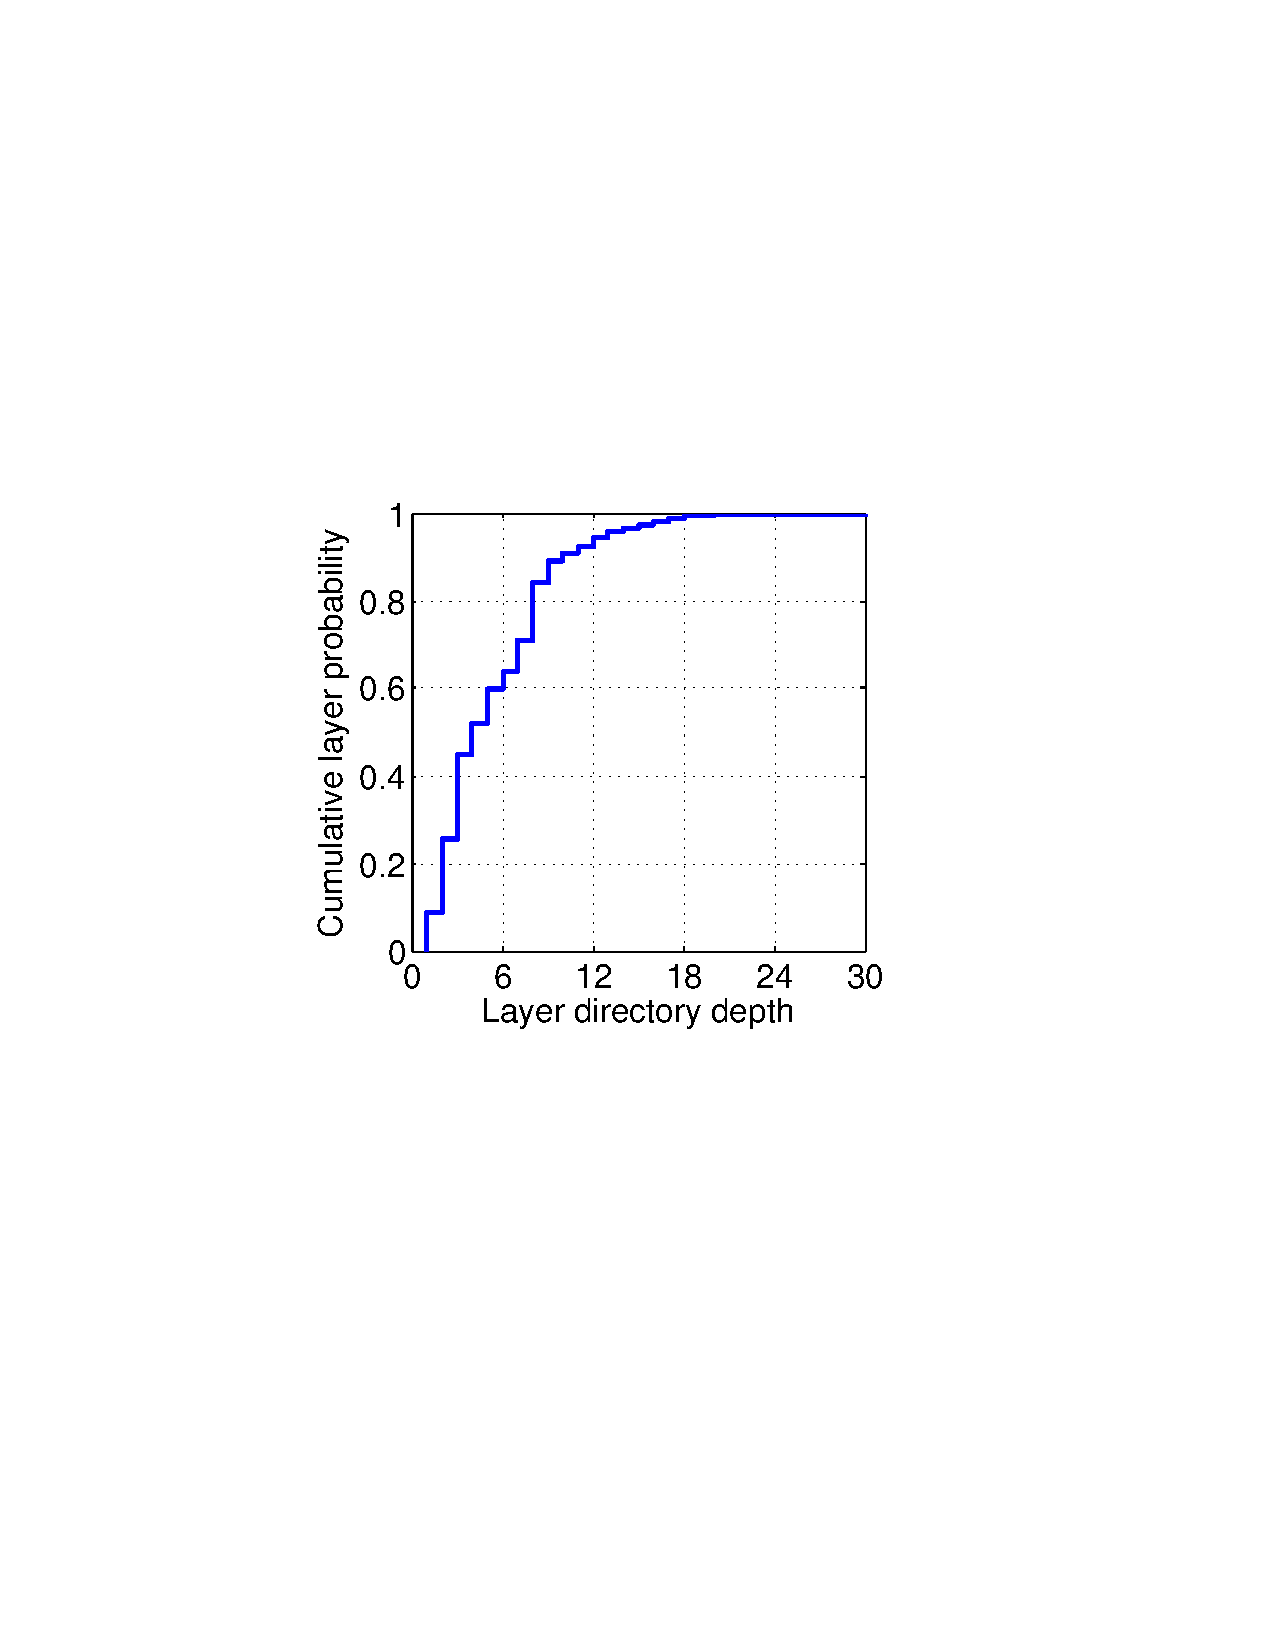
\includegraphics[width=0.23\textwidth]{graphs/layer_depth.pdf}
	}
	\subfigure[Histogram of layers by layer directory depth]{\label{fig_hist_layer_depth}
		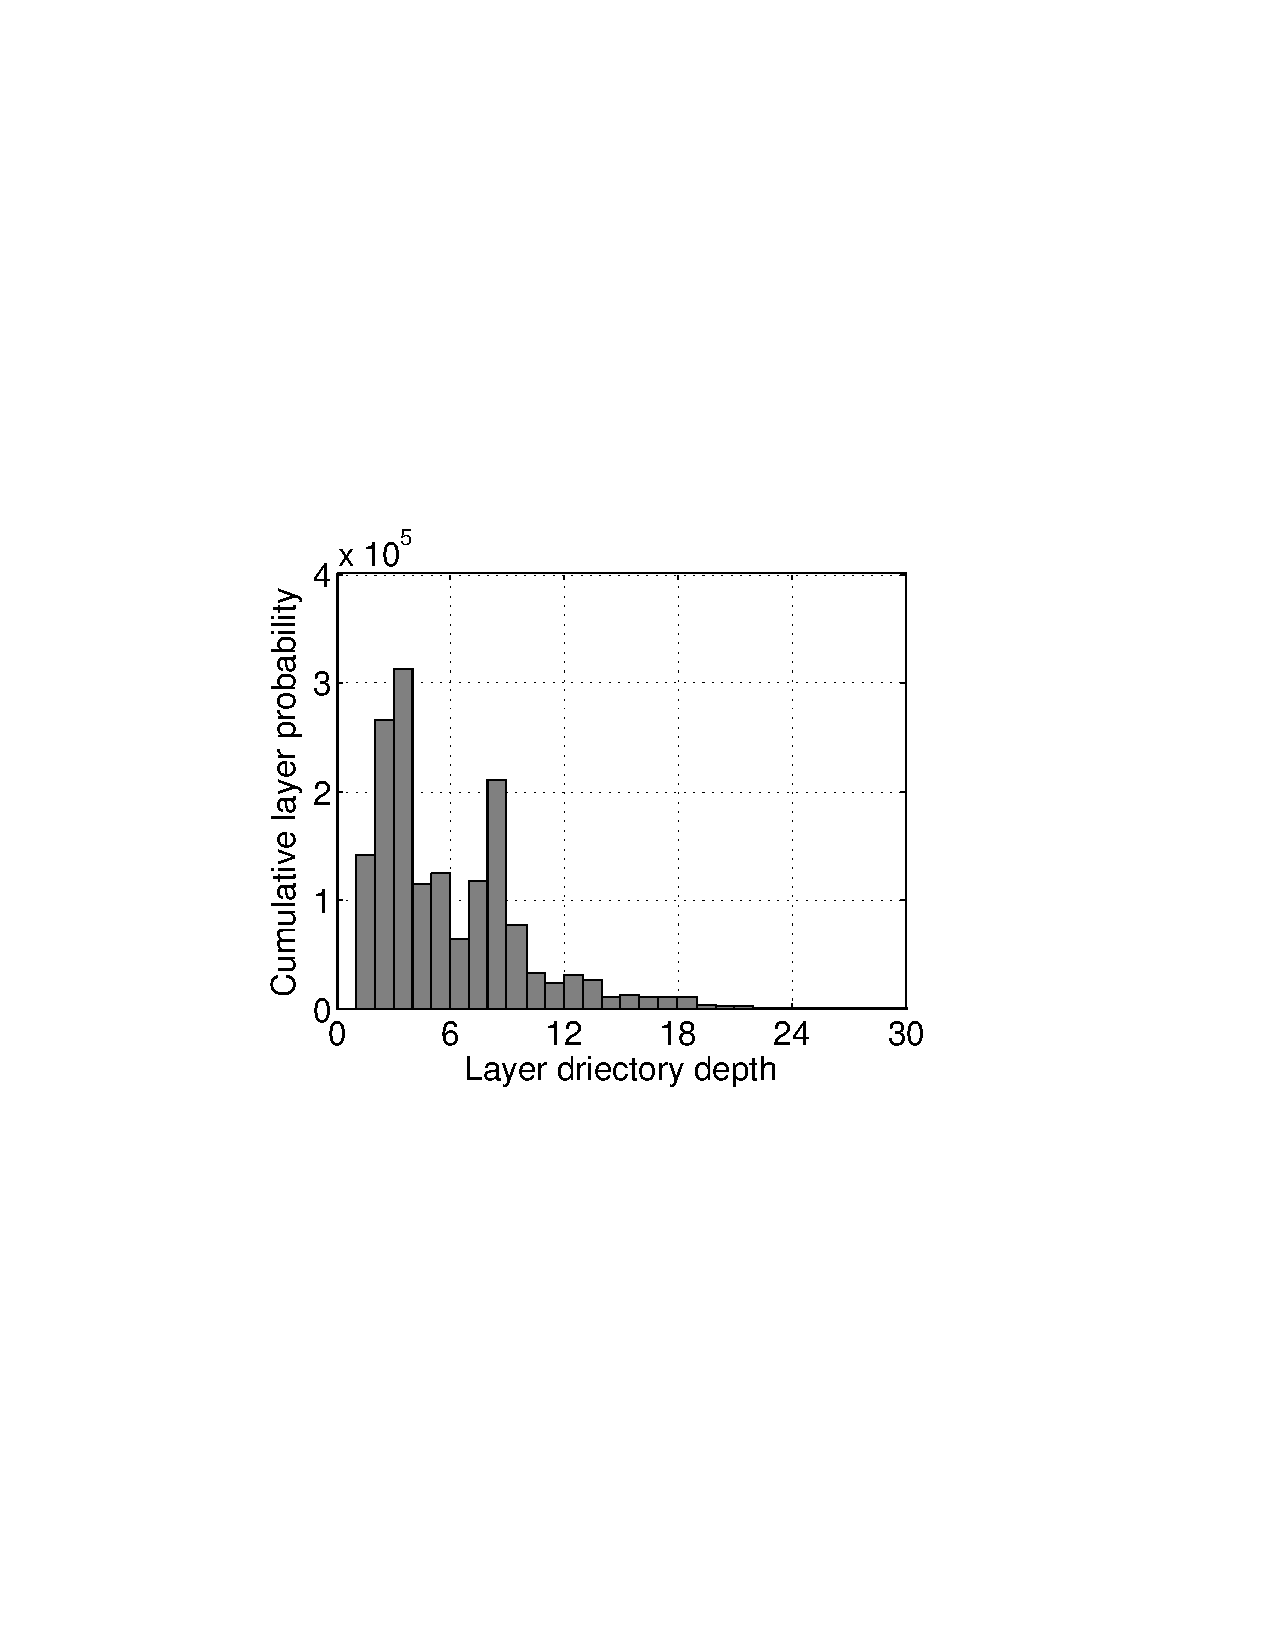
\includegraphics[width=0.22\textwidth]{graphs/hist_layer_depth.pdf}
	}
	\caption{Layer directory depth distribution}
	\label{fig-layer-dir}
\end{figure}

\subsection{Images}
\label{sec:images}

We continue analyzing images and present the following useful metric distributions: image size and compressibility, layer reference count, file and directory
counts. 

\paragraph{Image size}%{Layer and image size}

%80\% of images are less than 794 MB in uncompressed format
%80\% of images are less than 312 MB in compressed format
%
%50\% 406
%50\% 157

%\nancomment{add pdf if can}
%\acomment{Where is layers analysis when you say similarly? I wrote above
%para.. see for consistency.}
%Conatiner image size determines the runtime of container if it is not already
%cached locally. 
Similar to layers, we measured compressed and uncompressed image size. 
Figure~\ref{fig:image-size-cdf} show the image size distributions. 
%and a finer resolution only covering images smaller than 1.5 GB.
%\acomment{Could not locate the figures you are talking about. I see two figures
%layers size and image size.}
We find that 80\% of the images have an uncompressed size less than
794 MB and compressed size of 312 MB.
%while compressed images are less than 0.48 GB. 
In the median, this decreases to 406 MB and 157 MB, respectively. The largest
uncompressed image is 498 GB which is a Ubuntu-based image.  

\emph{Figure~\ref{fig:image-size-cdf} shows that the majority of uncompressed images in
Docker Hub are small which aligns with the Docker philosophy to package
software and distribute software in containers but include only its necessary
dependencies.}

\paragraph{Compression ratio}
%\begin{figure}
%	\centering
%	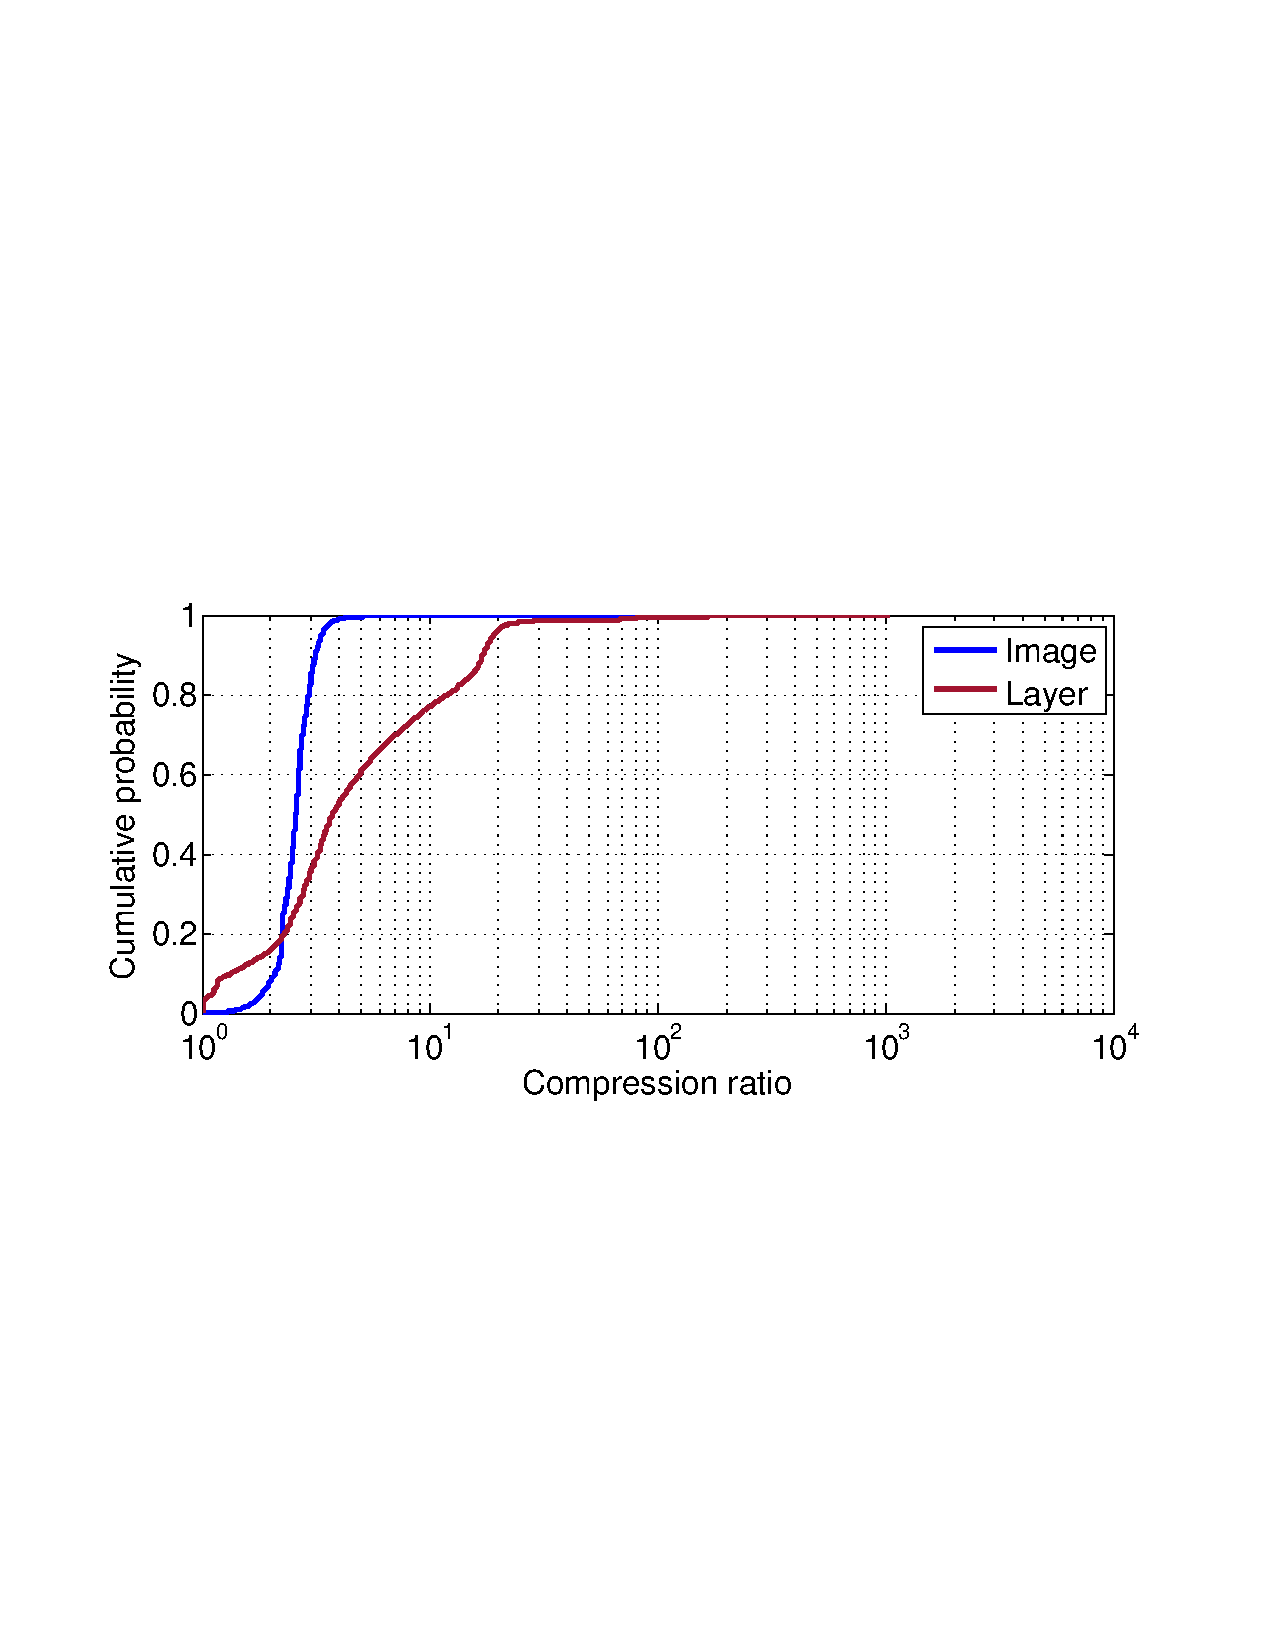
\includegraphics[width=0.4\textwidth]{graphs/compress-ratio-cdf.pdf}
%	\caption{CDF of compression ratio.
%	}
%	\label{fig:compress-ratio}
%\end{figure}

%\begin{figure}[!t]
%	\centering
%	\subfigure[Image compression ratio]{\label{fig_hist_image}
%		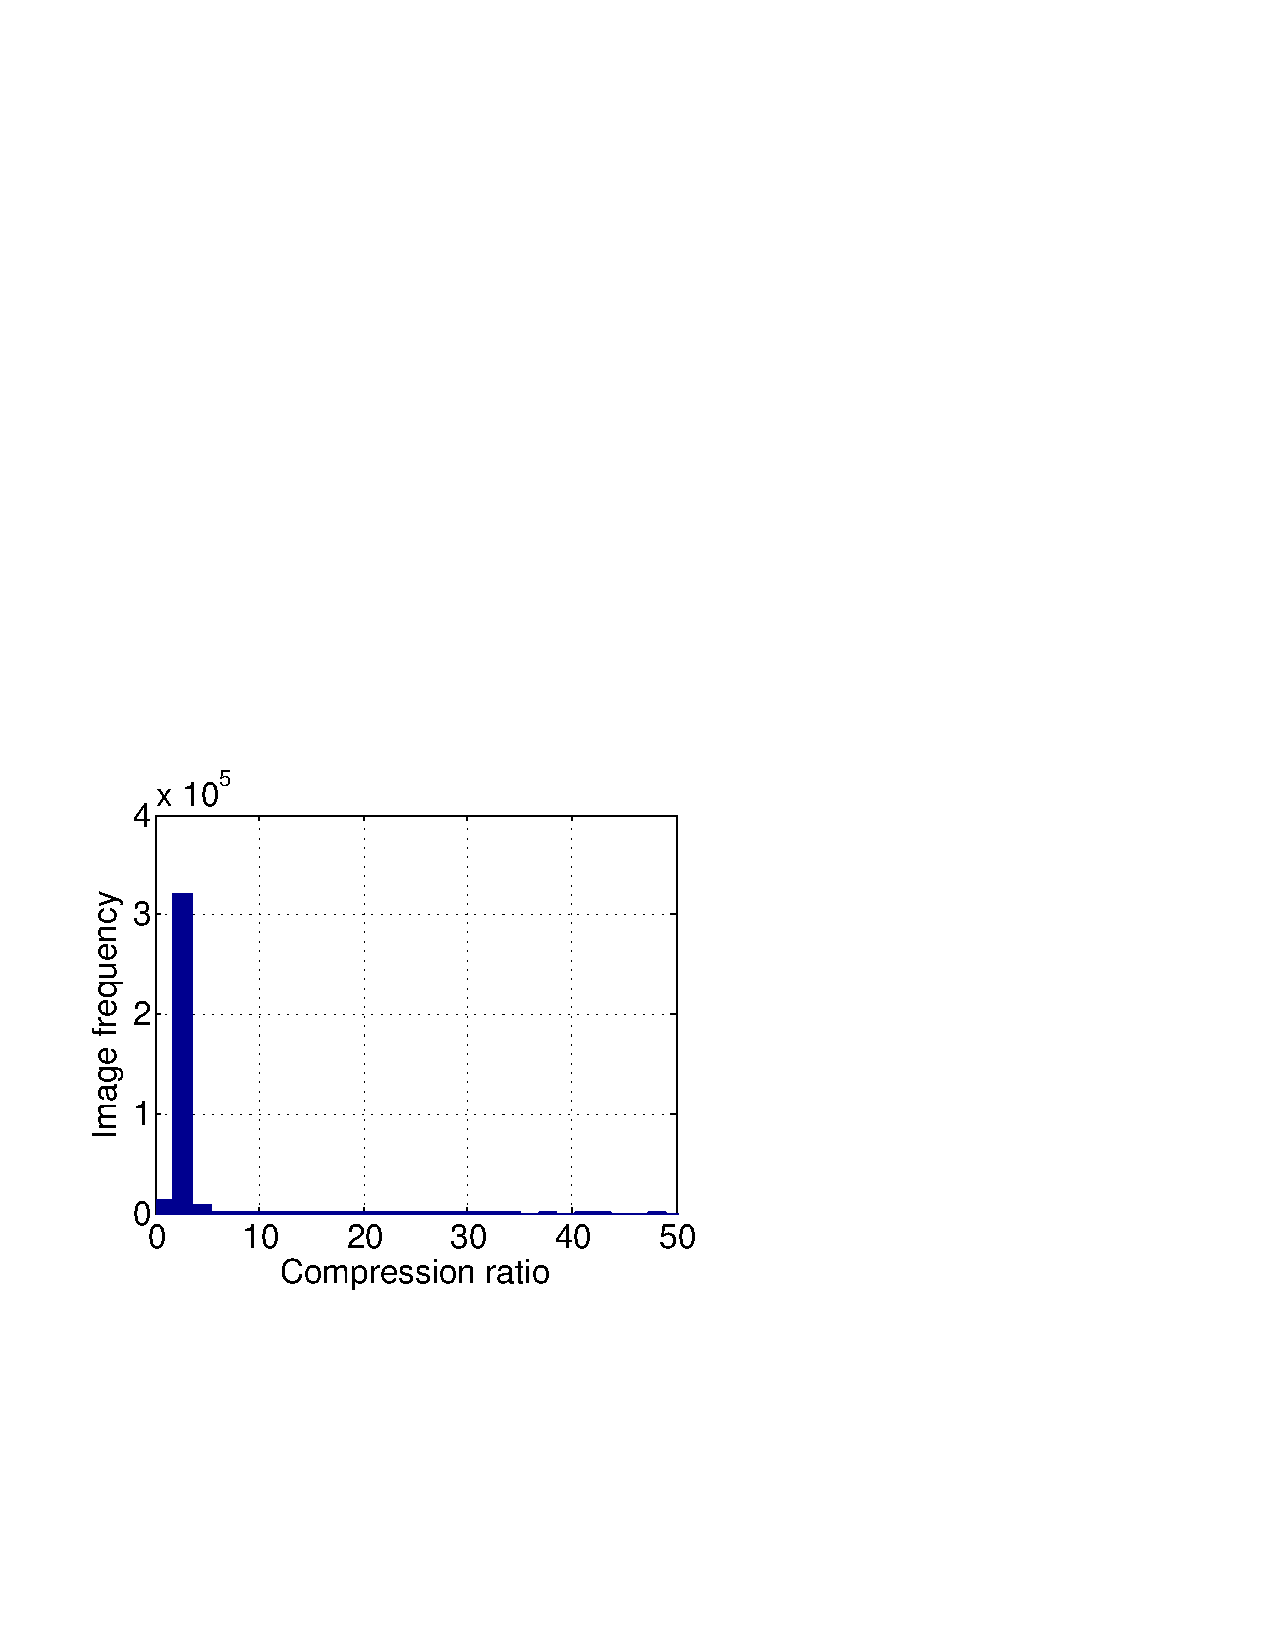
\includegraphics[width=0.215\textwidth]{graphs/image-compress-ratio-pdf.pdf}%
%	}
%	\subfigure[Layer compression ratio]{\label{fig_hist_layer}
%		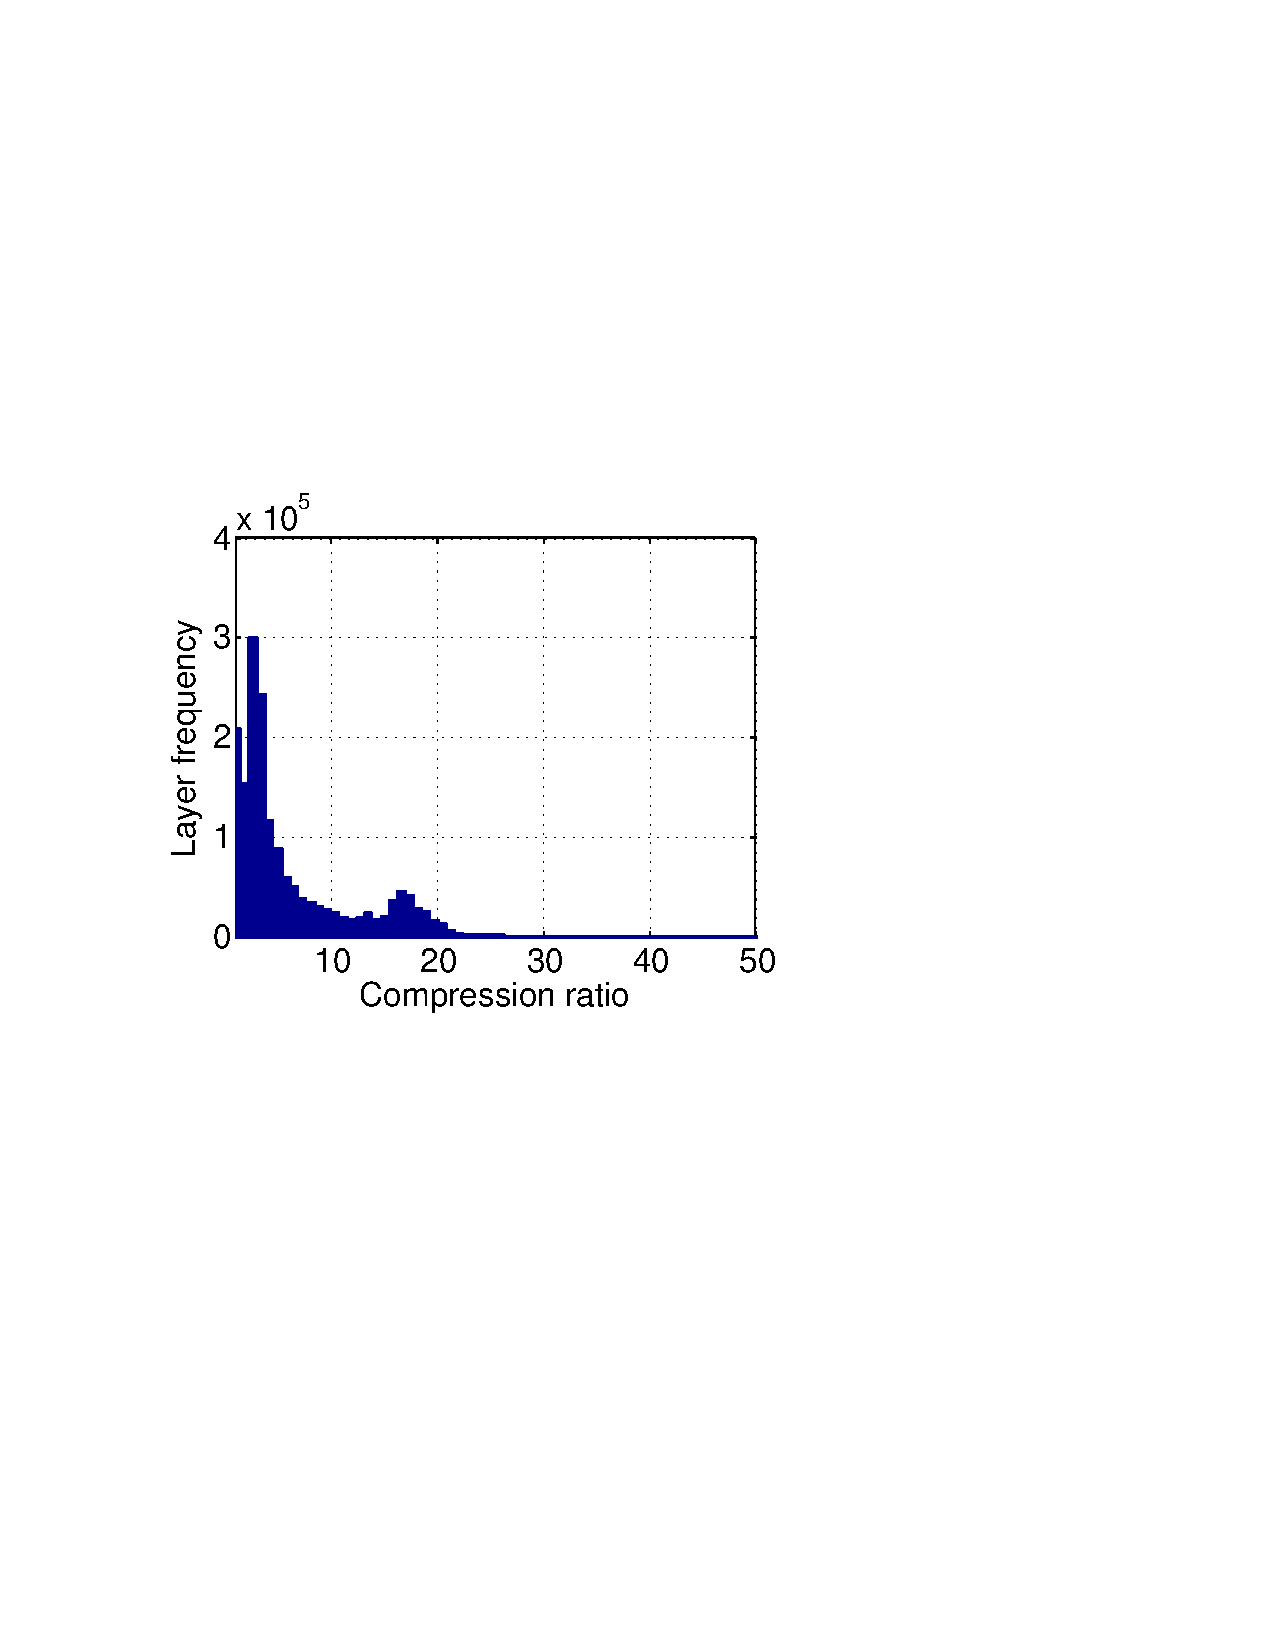
\includegraphics[width=0.22\textwidth]{graphs/layer-compress-ratio-pdf.pdf}
%	}
%	\caption{Histogram of image and layer compression ratio.}
%	\label{fig:reference-cnt}
%\end{figure}

%Figure~\ref{fig:compress-ratio} shows the compression ratio of the container
%images.    %\nancomment{there is redundancy and avg compression ratio}}

To further study the sizes and the impact of compression, we calculate the
compression ratios for images (see Figure~\ref{fig:compress-ratio}).
80\% of images have compression ratio less than 2.9 while the median is 2.6. 
\textit{We see that majority of images have a compression ratio within 2-3.}
Compare with compression ratio for layers, we see that images have a much smaller
compression ratio. 
\textit{This means that images contains both layers with high compression ratio and low compression ratio.}
%, which means images contains different layers and high . 

%\acomment{Found following para in directory count subsection..}
%
%The ALS-to-CLS ratio is generally greater than the FLS-to-CLS ratio because
%small files in layers get larger when combined in a tar archive.
%
%90\% of layers have a  compression ratio less than 4 and the median compression
%ratio is 2.6. The largest compression ratio is 1026.
%%
%Half of the layers have a compression ratio around 3.
%
%
%The maximum FLS-to-CLS is 512,930 and maximum ALS-to-CLS is 1026.
%
%Looking at the histogram (see Figure~\ref{}), we see
%that around 600,000 layers have a compression ratio of between 2 and 3 while
%more than 300,000 between 1 and 2.
%
%Two peaks in the graph correspond to 587,000 layers that have the FLS-to-CLS
%ratio of 3 and 331,000 layers that have the ALS-to-CLS ratio of 3.

\paragraph{Layer count per image}
%\nancomment{more layer more matedata? overhead for union fs}

\begin{figure}[!t]
	\centering
	\subfigure[CDF of layer count]{\label{fig:layer_count}
		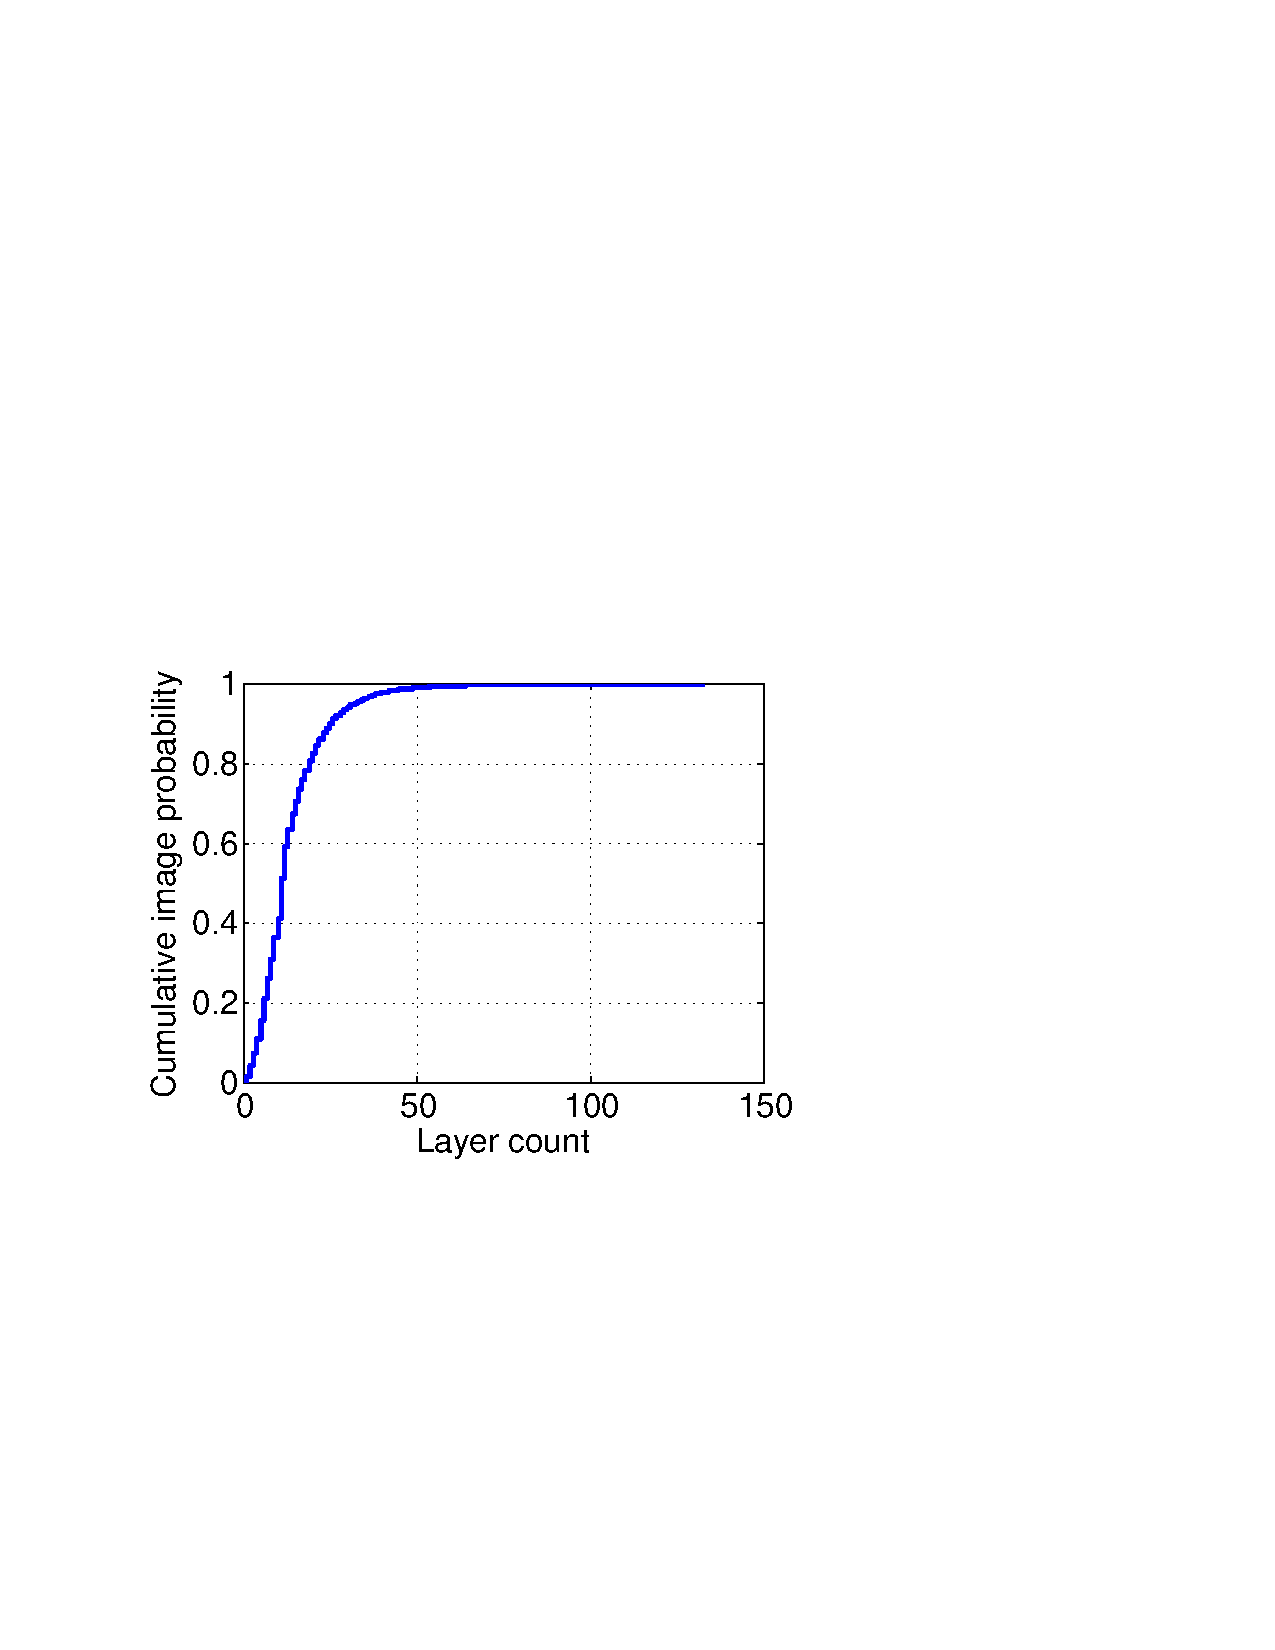
\includegraphics[width=0.215\textwidth]{graphs/image-layer-cnt}%
	}
	\subfigure[Histogram of layer count]{\label{fig:hist_layer_count}
		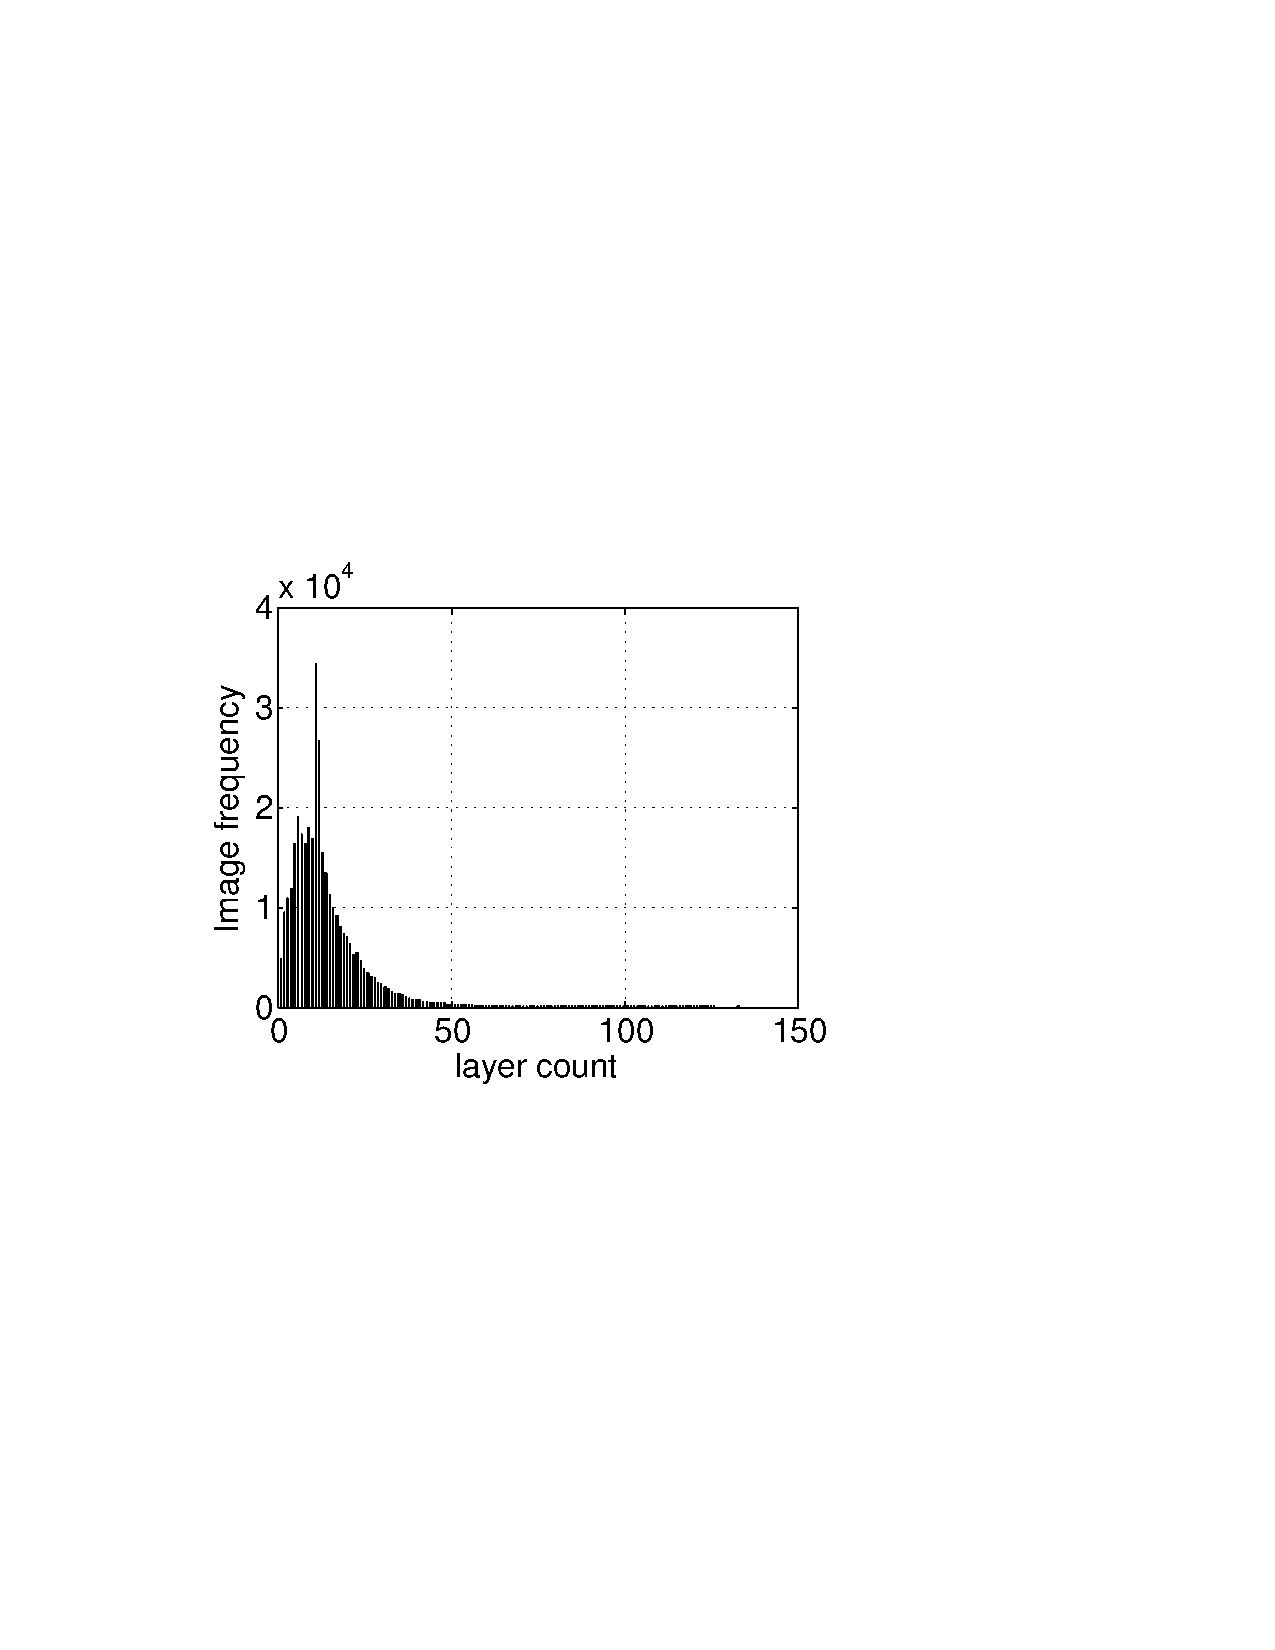
\includegraphics[width=0.21\textwidth]{graphs/image-layer-cnt-pdf.pdf}
	}
	\caption{CDF and histogram of Layer count per image.}
	\label{fig:image-size}
\end{figure}

As discussed in~\ref{sec:layers}, images consist of a set of layers.
It is important to understand the layer count of the images as previous
work found that the number of layers can impact the performance of
I/O operations~\cite{slacker}. Therefore, we count the number of layers
per image and plot the CDF (see Figure~\ref{fig:layer_count})
and layer count frequencies (see Figure~\ref{fig:hist_layer_count})for all
Docker Hub images.

The results show that 90\% of the images have less than 26 layers while
half of the images have less than 10 layers. 11 layers is also the most
frequent layer value with 34,420 images consisting of exactly 11 layers.
The maximum layer count is 120 in the \textit{cfgarden/120-layer-image}.
We also find that there are 4,792 images which only consist of a single layer.

\emph{As a rule of thumb, less number of layers is better for the union file
	system as it then needs to handle less metadata. However, as a tradeoff,
	reducing the number of layers significantly effects the data sharing among images.
	%As a result, we see less number of layers shared among different images.
	For an example, if a image consists of only single layer its data can not be shared
	with other images.}
%\begin{figure}[!t]
	\centering
	\subfigure[CDF of layer reference count]{\label{fig_repeate_layer}
		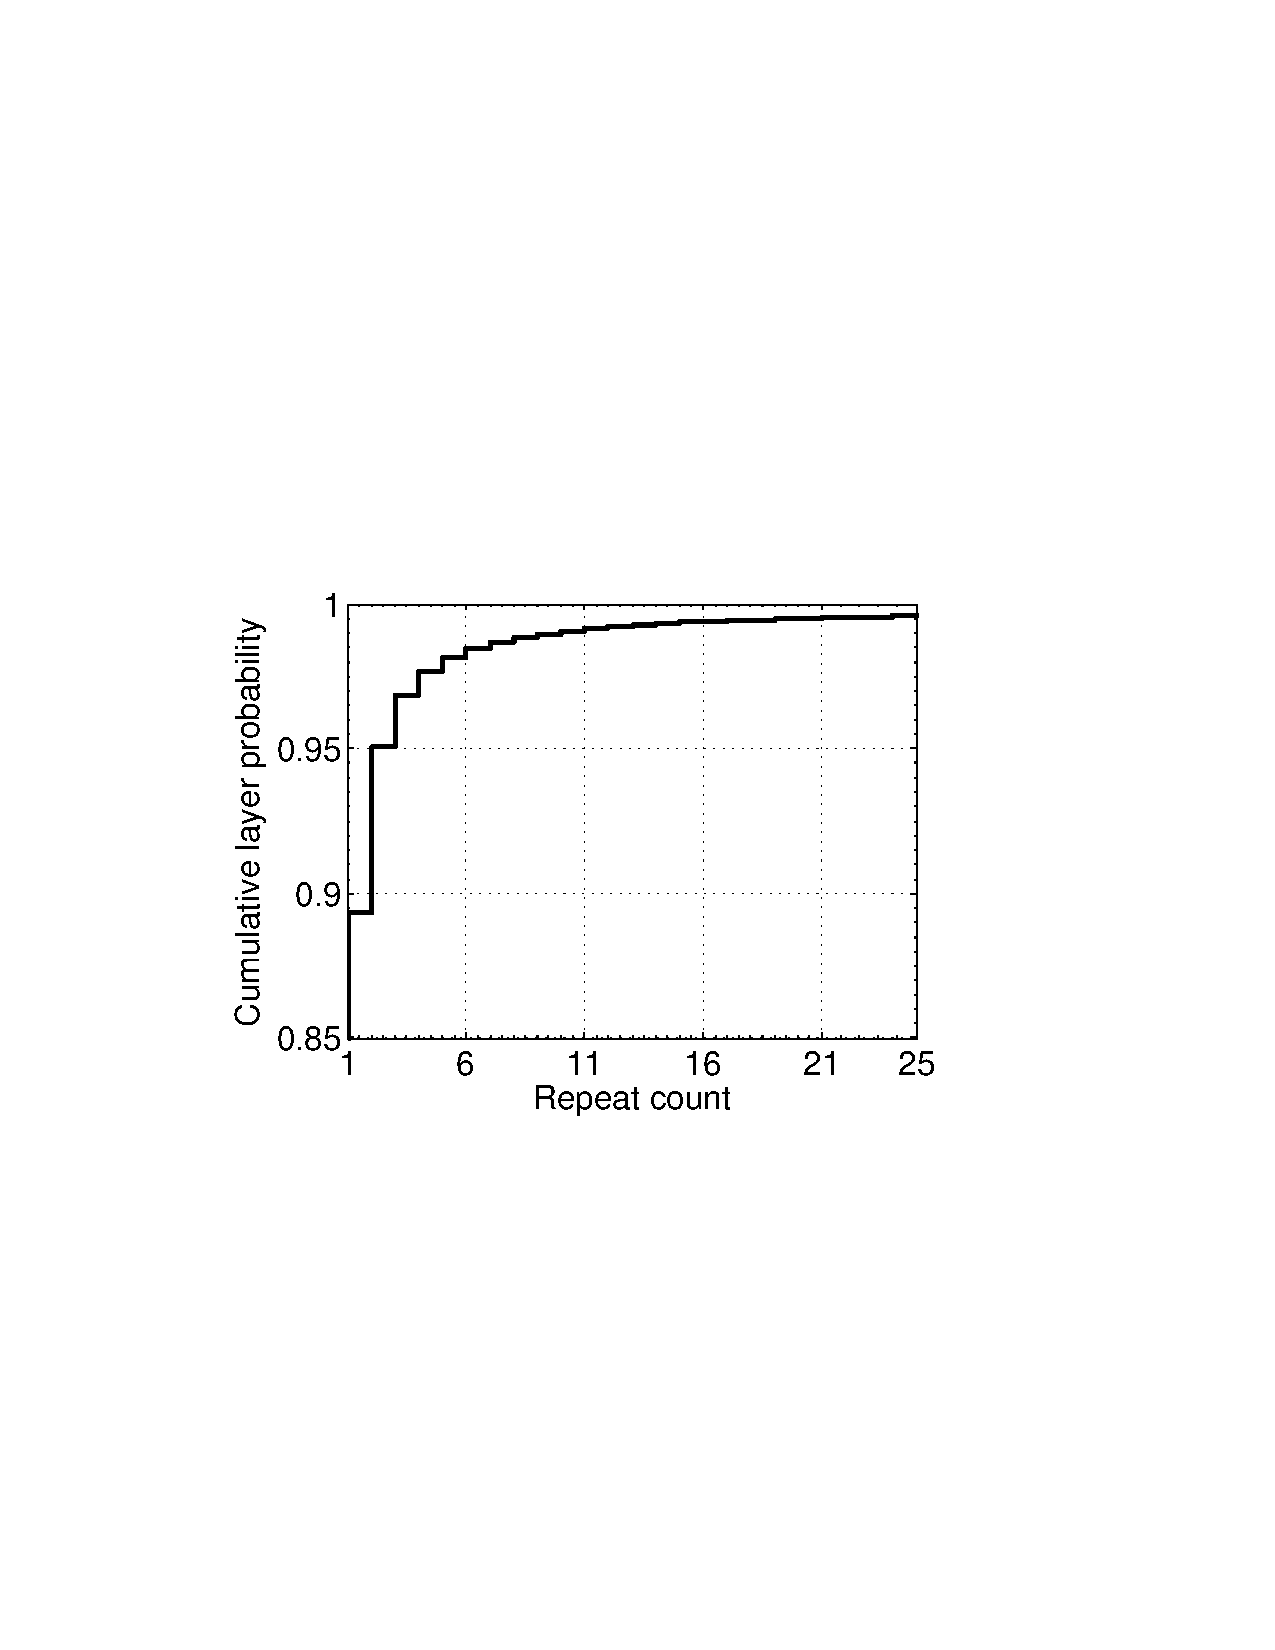
\includegraphics[width=0.23\textwidth]{graphs/repeate_layer.pdf}
	}
	\subfigure[Histogram of layer reference count]{\label{fig_hist_repeate_layer}
		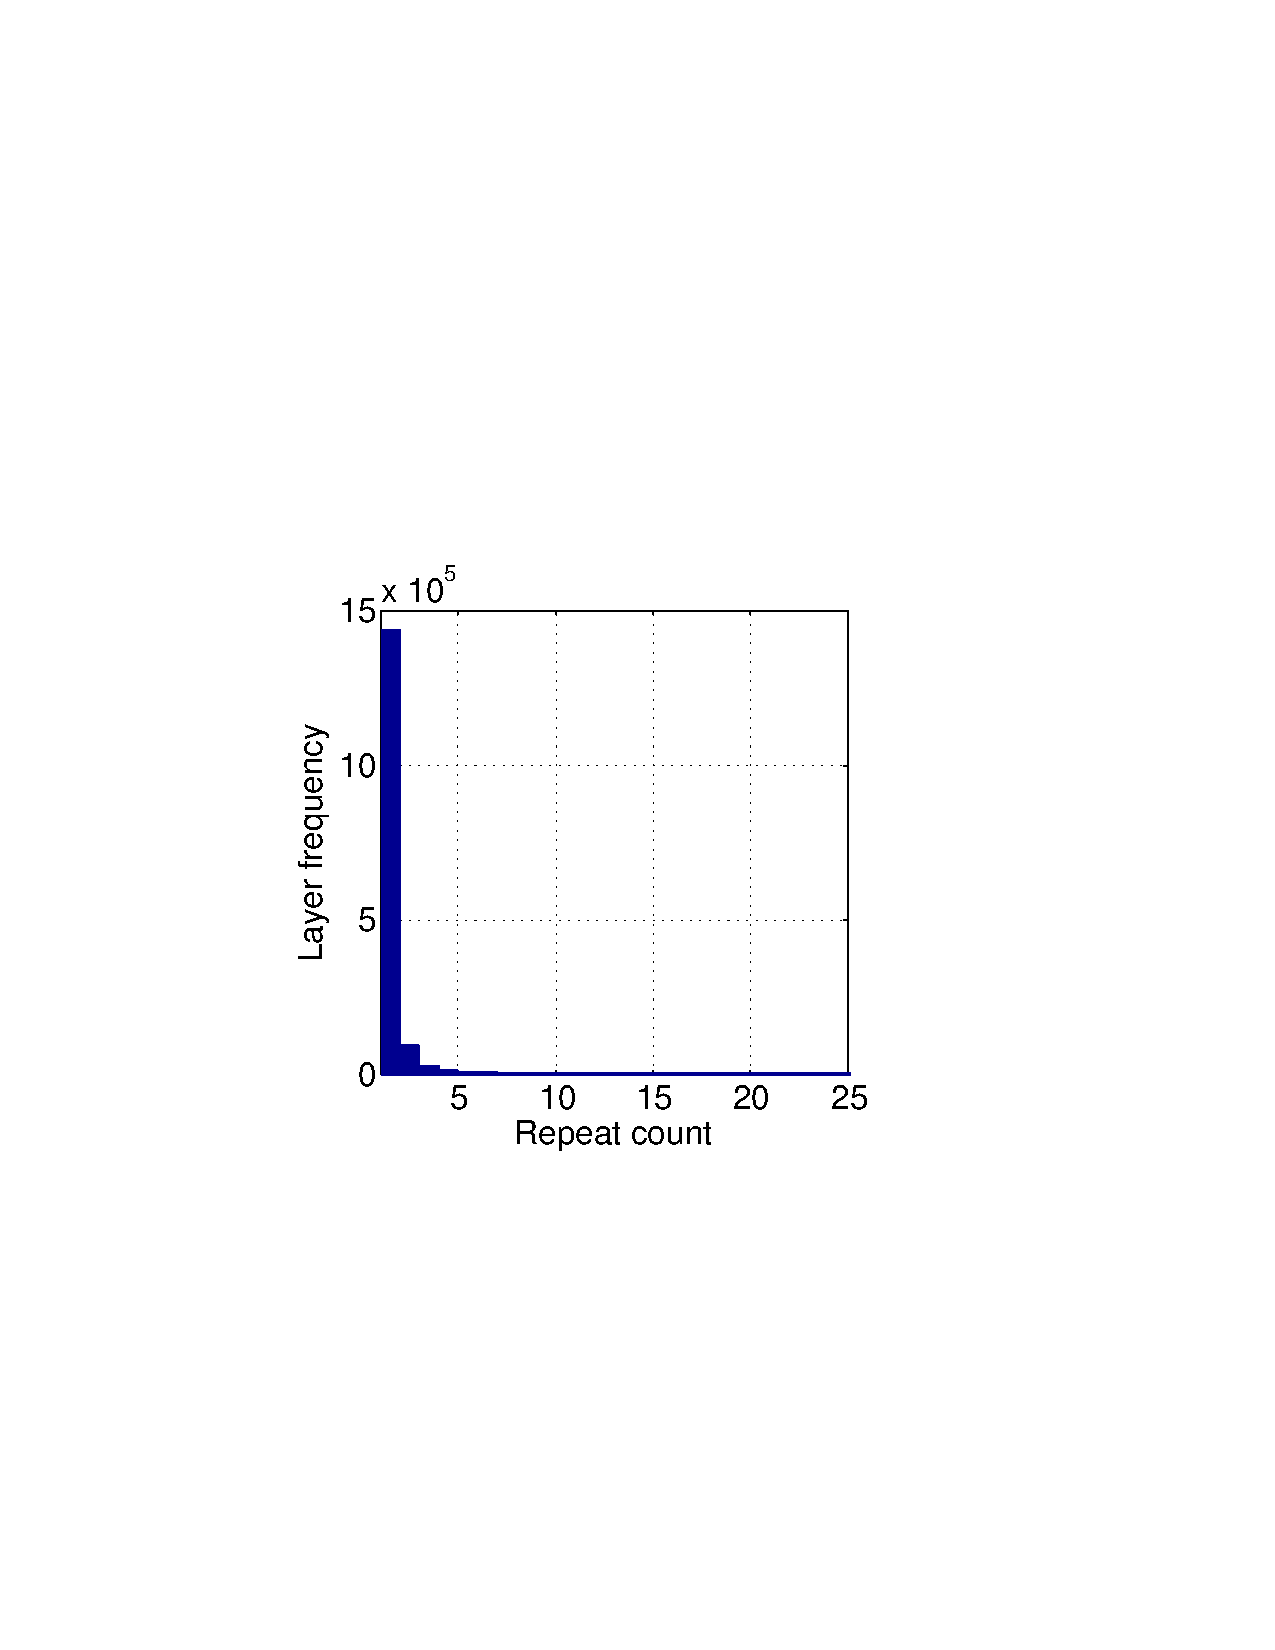
\includegraphics[width=0.223\textwidth]{graphs/hist_repeate_layer.pdf}
	}
	\caption{Layer reference counts across all images}
	\label{fig-repeat-layer-cnt}
\end{figure}

%\paragraph{Repeat layer count distribution}
\paragraph{Layer reference count}
%\nancomment{should create more shared layers to remove duplicates}

\begin{figure}
	\centering
	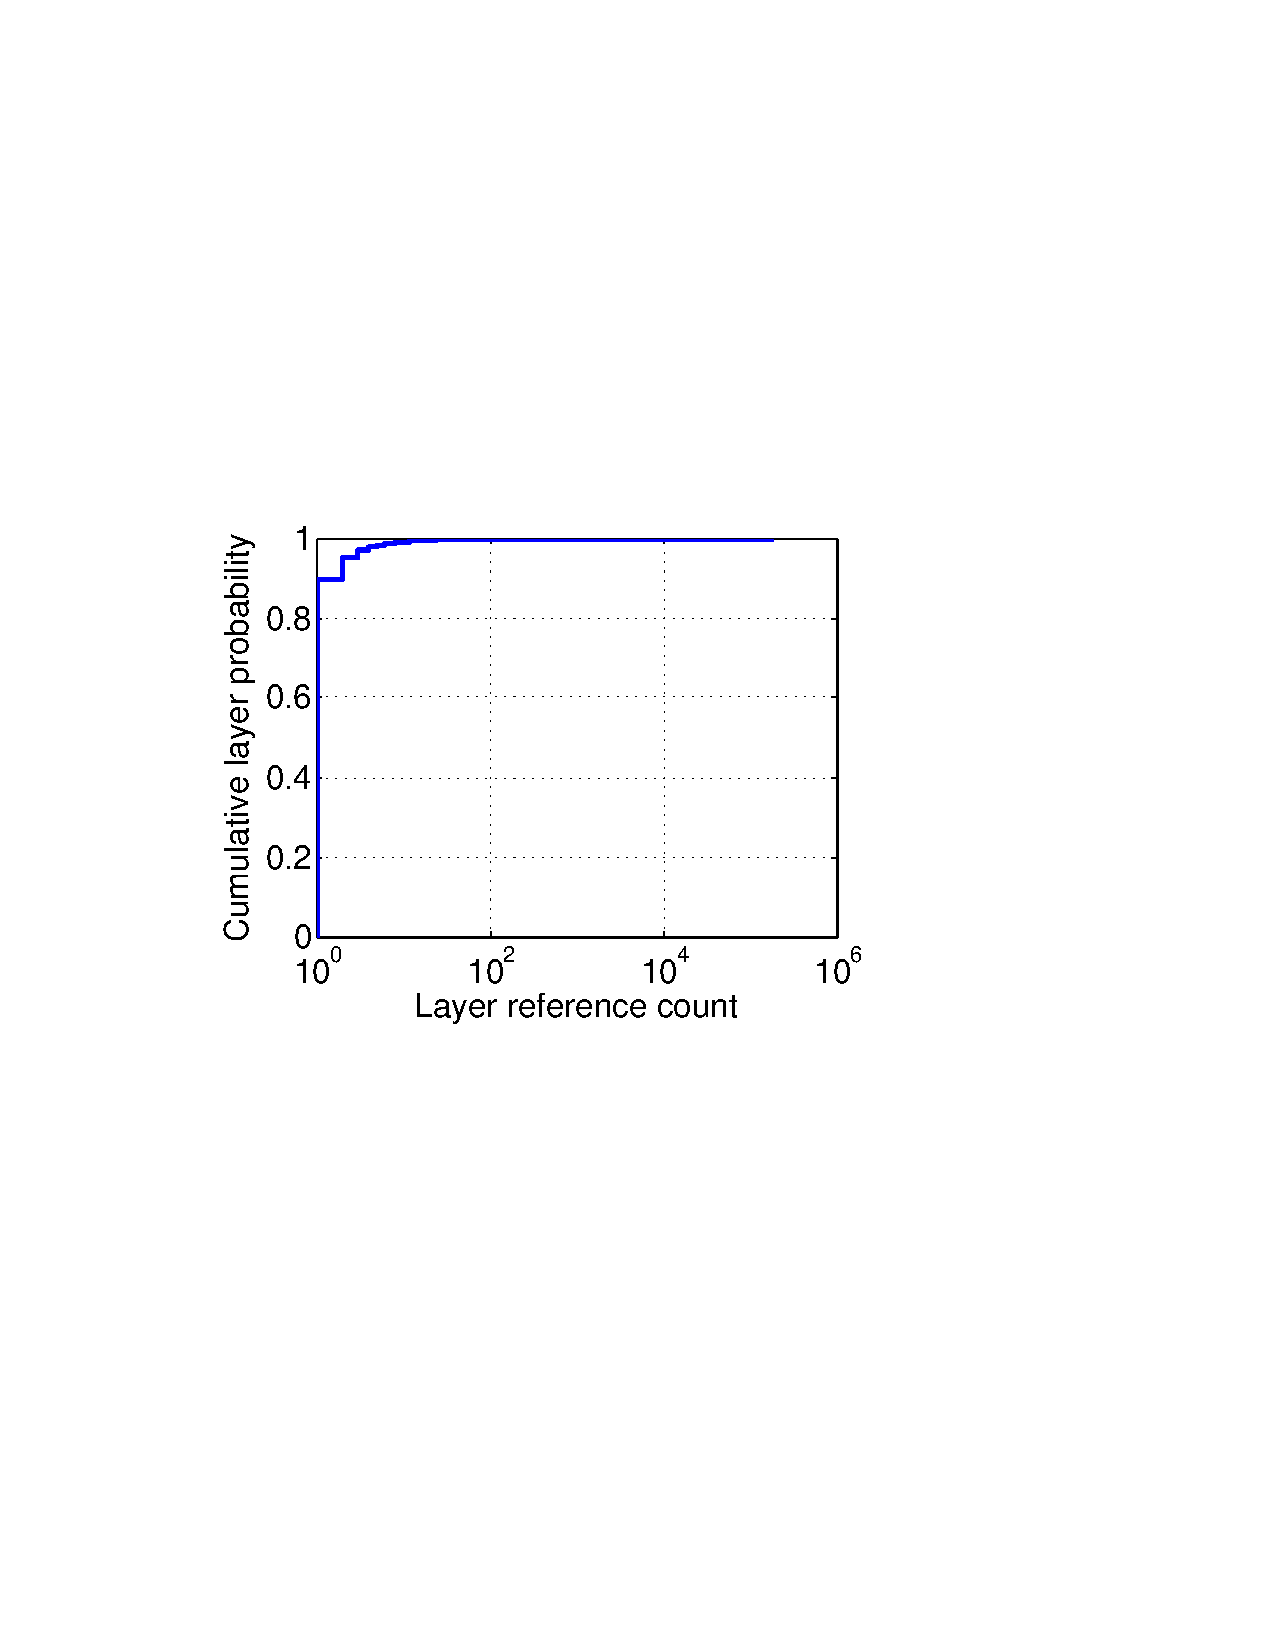
\includegraphics[width=0.21\textwidth]{graphs/shared-cnt-cdf.pdf}
	\caption{CDF of layer reference count.
	}
	\label{fig:ref_count}
\end{figure}

An interesting question is what is the sharing rate of layers across images.
We analyze all image manifests and count for each layer, how many times it is
referenced by an image. Figure~\ref{fig:ref_count} shows that around 90\% of
layers are only reference by a single image while 95\% are reference by not
more than 2 images. Similarly, 99\% of layers are shared among less than 25
images. 
%Figure~\ref{} shows the absolute values, revealing that
%almost 1.5 million images are only referenced once.  \acomment{Figure is
%	missing} While there is again a large spectrum of reference counts, the maximum
%is 33,428, the vast majority of layers is not shared. 
This hints that the
layer-based approach to improve storage efficiency is barely utilized and there
is room for improvement in how to construct more sharable layers.

\emph{These findings reveal that layer level CAS has not been very successful
	and most of the layers that exists in Docker Hub are not shared among images.
	Hence, there is a dire need of a better redundancy management.}

%89\% of 1
%95.1\% 2

\paragraph{Directory count and File count}

Next, we look at the directory (Figure~\ref{fig:dir-cnt-cdf}) and file count
(Figure~\ref{fig:file-cnt-cdf}) in images to determine if deploying images requires
handling of large amounts of metadata. 
Looking at directories, we see that 50\% of images have less than 3,326 directories and 90\% of images have less than
9,692 directories. %70\% of images have more than 2,500 directories. 
For
files, 50\% of images have less than 27,194 files and 90\% of images have less than 74,266 files.

This is consistent with our analysis of layer-based file and directory counts
and the number of layers per image. Again, \textit{we conclude that most images do not
require an extensive amount of metadata when being deployed as file and
directory counts are low except for few outliers.}

%This is consistent with our analysis of layer-based file and directory counts
%and the number of layers per image. Again, we conclude that most images do not
%require an extensive amount of metadata when being deployed as file and
%directory counts are low except for few outliers.

%\begin{figure}[!t]
	\centering
	\subfigure[CDF of compression ratio]{\label{fig_cdf_compression_ratio}
		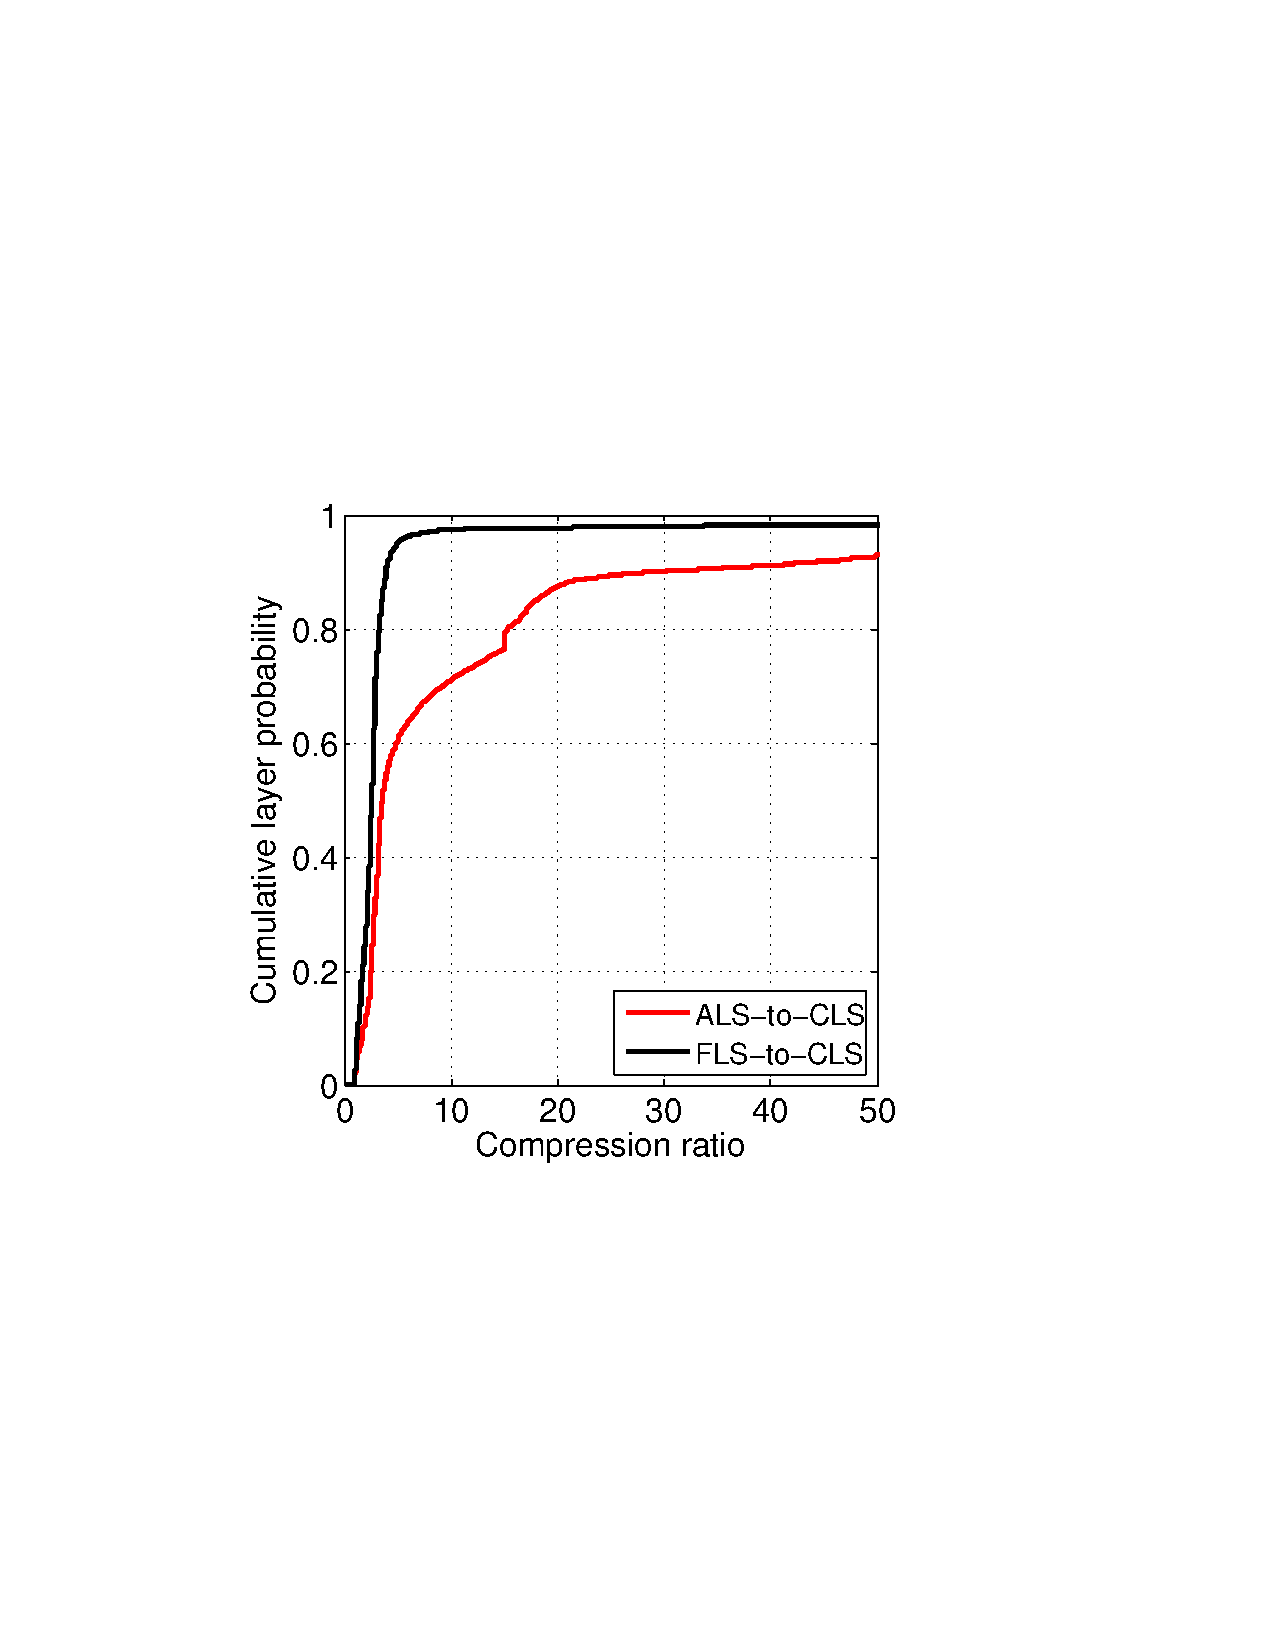
\includegraphics[width=0.23\textwidth]{graphs/cdf_compression_ratio.pdf}
	}
	\subfigure[Histogram of comp. ratios]{\label{fig_his_compression_ratio}
		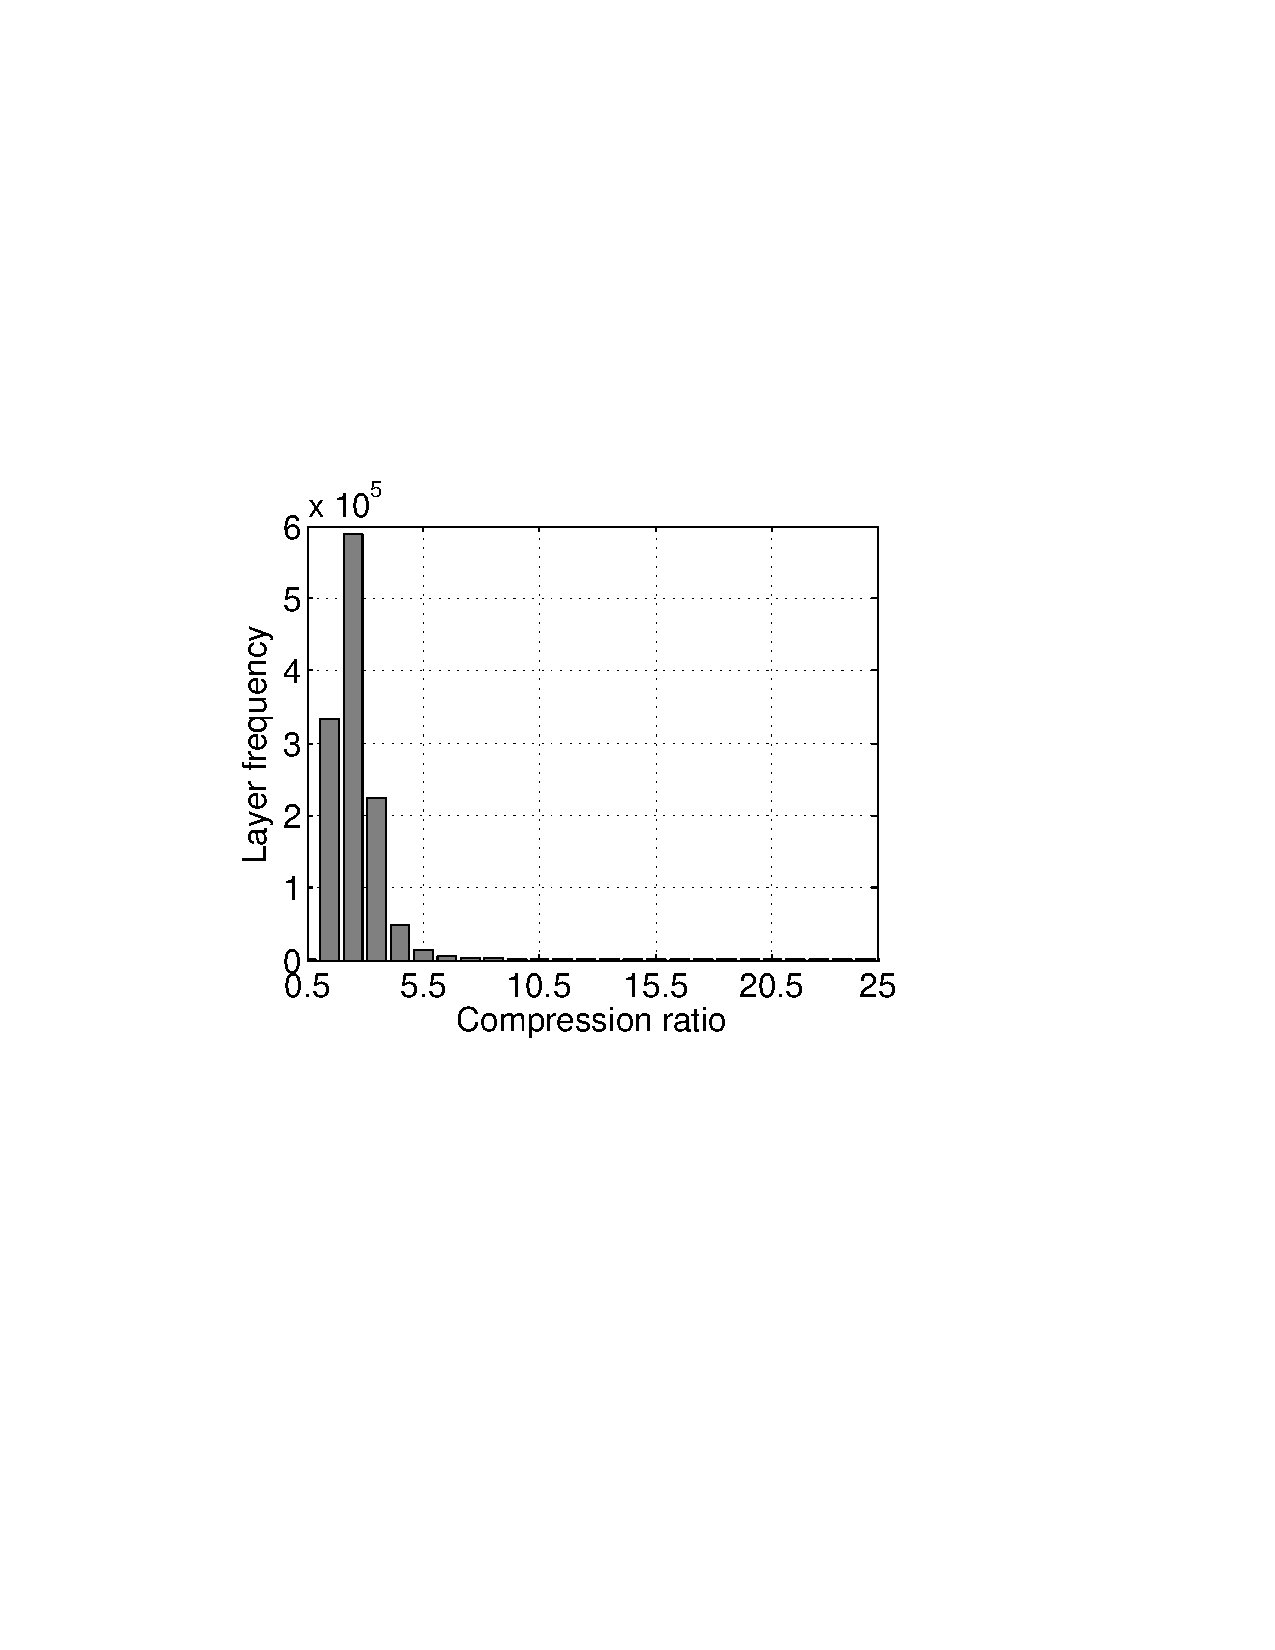
\includegraphics[width=0.223\textwidth]{graphs/his_compression_ratio.pdf}
	}
	\caption{Layer compression ratio distribution
	%\vcomment{Different colors are used in figure (a) and (b) FLS/CLS\nancomment{will address later}}
	}
	\label{fig-compression-ratio}
\end{figure}


%\paragraph{Layer compression ratios}

